\begin{refsection} 
 
\chapter{Solar Cells}\label{chapter:solar} 
 
\setlength{\epigraphwidth}{3in} 
\epigraph{\textit{``We are star stuff harvesting sunlight.” }}{Carl Sagan} 
\vspace{3em} 
 
Solar cell technology is a rapidly developing field, largely driven by the 
discovery of cheaper and more efficient materials. However, the conventional 
search for potential absorber layers in photovoltaic devices is expensive and 
time consuming. Modern high-throughput computational methods have the power to 
screen large amounts of materials relatively quickly, providing valuable 
information that allows experimental work to focus on promising compounds. In 
order to accurately screen materials, a proper selection metric is required. 
The Spectroscopic Limited Maximum Efficiency (SLME) attempts to improve upon 
the traditional Shockley-Queisser (SQ) limit by including the first-principles 
calculated absorption spectrum of the material in the determination of the 
efficiency. It also allows researchers to determine the thickness dependency 
of the efficiency, which is particularly interesting for thin-film solar cell 
research. \\ 
 
This chapter starts by explaining the basic working principles of a solar cell 
in Section~\ref{sec:slme-basics}. Next, Section~\ref{sec:slme-metric} 
continues by discussing the SLME, as well as its predecessor, the Shockley 
Queisser limit. In Section~\ref{sec:slme-CuAu}, this selection metric is 
applied to compare the potential of a range of ternary I-III-VI$_2$ compounds 
in both the CuAu-like and the chalcopyrite phase. Finally, some crucial 
aspects of our chosen selection metric are investigated in 
Section~\ref{sec:slme-analysis}. 
 
\pagebreak 
 
\section{Introduction} 
 
Nearly all sources of energy found on earth are in some way derived from the 
sun. Both animals and plants depend on solar energy to produce the heat and 
sustenance they need to survive. Fossil fuels are nothing more than long 
buried organisms, exposed to millions of years of heat and pressure in the 
earth's crust. Wind energy would not exist without the air currents that are a 
product of solar heated air and the rotation of the earth. Solar cells are 
\textit{PhotoVoltaic} (PV) devices that try to directly convert the sun's 
light into electricity, by absorbing the incoming photons and using the 
resulting energy to create a current of moving electrons. They have the 
advantage of being a renewable source of clean energy, whose application can 
be much more distributed than more conventional sources of 
electricity~\cite{Marsden2011}. 
 
The first practical photovoltaic devices were constructed in the 1950s. Over 
the course of the next decades, solar cell technology was mainly developed by 
the space industry, which required a reliable source of energy for its 
satellite applications. In the 1980s, solar cells received an increased amount 
of attention due to the oil crisis and a growing demand for power supply in 
remote areas that are not connected to the electricity grid. More recently, 
the threat of global warming has expanded the interest in sustainable energy 
sources. Advances in technology have increased the efficiency and longevity of 
solar cells, while reducing the costs of production and maintenance. 
Governments around the world have started initiatives to increase the 
percentage of the world's renewable energy supply. 
Figure~\ref{fig:slme-pv_evo} shows the results of these efforts. We can see 
that the PV market has increased significantly over the past decade, now 
contributing 5.9\% of the total global (grid-connected) energy production. 
 
Although the growth of the PV market is promising, continued efforts must be 
made to increase the share of renewable energy in the global energy 
production. In order to make solar cells more economically competitive with 
conventional sources of electricity, new materials have to be found that 
either increase the efficiency or lower the cost of PV devices. In this 
chapter, we investigate a selection metric that determines the potential of a 
material for solar cell applications. 
 
\begin{figure}[!htp]  
\centering 
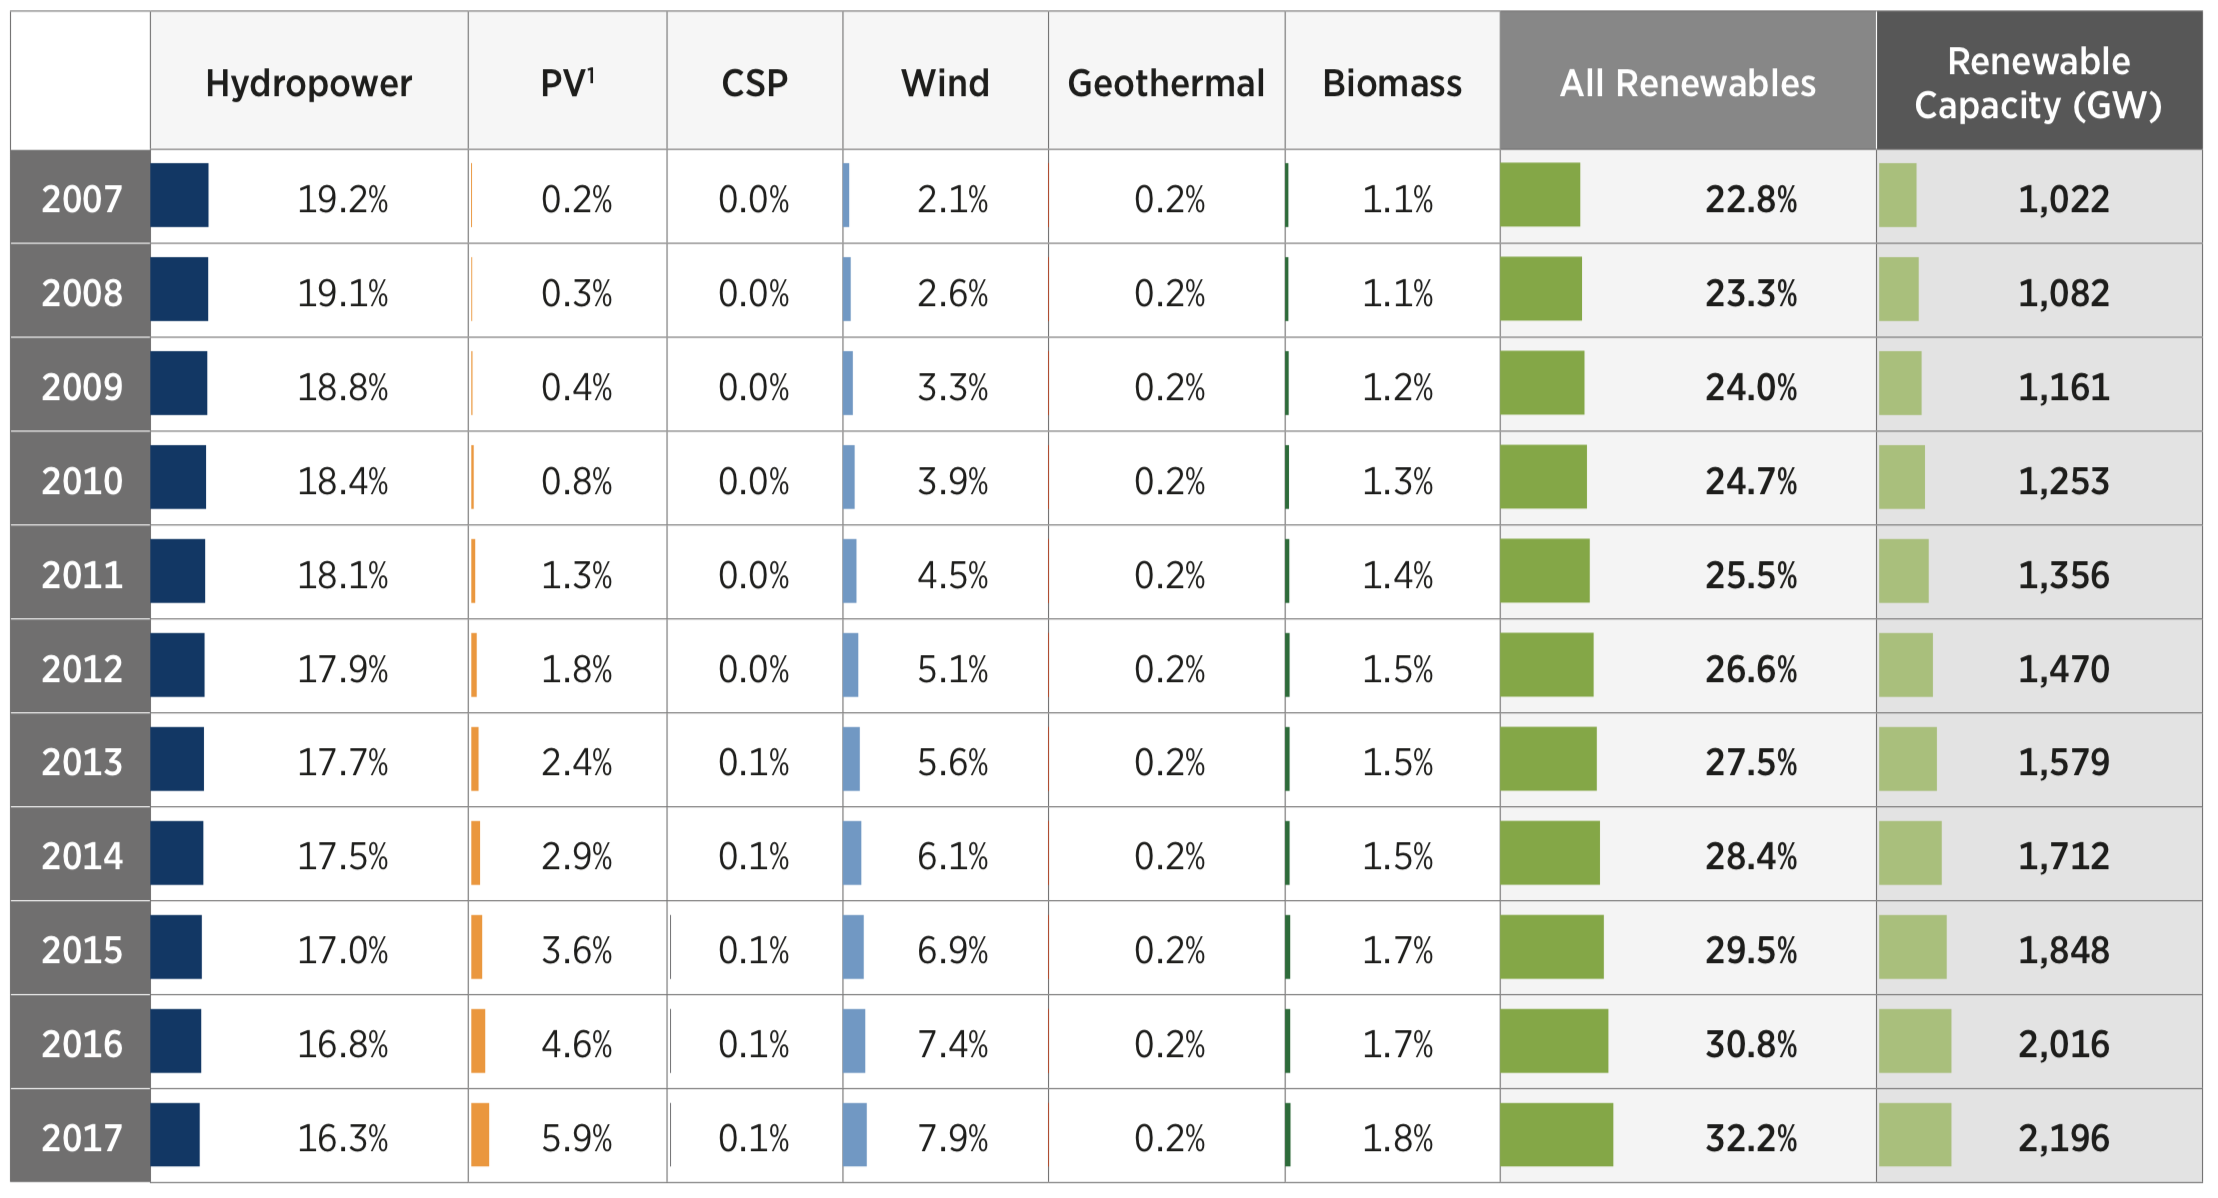
\includegraphics[width=0.8\textwidth]{./Figures/slme/pv-evo.png} 
\caption{Renewable electricity as a percentage of the total installed global 
electricity capacity. Note that the PV numbers here are for grid-connected production only, represented by the index 1. CSP stands for concentrated solar power. Taken from~\cite{NREL2017}.} 
\label{fig:slme-pv_evo}  
\end{figure} 
 
 
% 
%The Shockley-Queisser limit~\cite{Shockley1961} is one of the most well-known 
metrics to determine the maximum efficiency an absorber material can produce 
in a single-junction solar cell. It was proposed in 1961 and provides a direct 
relation between the band gap of a material and its maximum possible 
efficiency. More recently, Yu and Zunger expanded on the work of Shockley and 
Queisser by introducing the Spectroscopic Limited Maximum 
Efficiency~\cite{Yu2012} (SLME), which takes the absorption coefficient and 
thickness into consideration for the calculation of the maximum efficiency. 
The SLME has since been used to investigate the potential of photovoltaic 
absorber materials such as perovskites~\cite{Meng2016}, direct band gap 
silicon crystals~\cite{Lee2014}, chalcogenides, and other materials. In our 
recent work on CuAu-like~\cite{Bercx2016} and Stannite~\cite{Sarmadian2016} 
structures, we also used the SLME to study the efficiency of these materials 
in the context of thin film solar cells. Interestingly, we found several 
materials with an SLME above the Shockley-Queisser limit, and identified that 
this is due to the lower recombination current obtained for the material at 
lower thicknesses. 
 
 
\section{Solar Cell Basics} \label{sec:slme-basics} 
 
This section discusses the basics of solar cells, starting from a presentation 
of the solar spectrum and the absorption coefficient. It continues by 
explaining recombination effects, an important limiting factor for solar cell 
efficiency. The P-N junction, as well as the relevant equations, are the next 
topic of this section. Finally, we present the working principles of the solar 
cell, as well as a discussion of its I-V characteristic, which is essential 
for understanding the selection metrics introduced in the 
Section~\ref{sec:slme-metric}. 
 
\subsection{Solar Spectrum} 
 
Before discussing the operation of solar cells, we briefly take a look at the 
solar spectrum itself (Fig.~\ref{fig:slme-solar}). In good approximation, the 
sun emits electromagnetic radiation as a black body, a perfectly absorbing 
mass whose emission spectrum is determined by Planck's radiation 
law~\cite{Planck1901}. Due to the influence of the sun's atmosphere, the 
spectral distribution that reaches the outside of earth's atmosphere differs 
from the ideal black-body spectrum. Before reaching the planetary surface, the 
incoming radiation intensity is further attenuated by various scattering and 
absorption effects~\cite{Bird1986}. The degree of attenuation depends on the 
angle at which the light enters the atmosphere. The solar spectra are usually 
classified by their \textit{Air Mass} (AM)~\cite{Green1981}: 
\begin{minipage}{1\textwidth} 
\begin{minipage}{0.4\textwidth} 
\begin{equation} 
\text{Air Mass} = \frac{1}{\cos \theta_z}, 
\end{equation} 
\end{minipage} 
\begin{minipage}{0.6\textwidth} 
\centering 
\includegraphics[width=1\textwidth]{./Figures/slme/am2.png} 
\captionof{figure}{\label{fig:slme-Airmass}Relation between zenith and Air 
Mass. \cite{Newport}} 
\end{minipage} 
\end{minipage} 
\vspace{0.2in}\\ 
where $\theta_z$ is the zenith angle of the incoming 
light~(Fig.~\ref{fig:slme-Airmass}). The use of these standard spectra allows 
the performance of devices to be judged fairly, by exposing them to the same 
agreed-upon spectrum. In this work, we use the AM 1.5G irradiance spectrum for 
all of our calculations, where `G' stands for global tilt. The global tilt 
refers to the angle between the normal of the surface and the direction of the 
incoming sunlight. 
 
\begin{figure}[!htp]  
\centering 
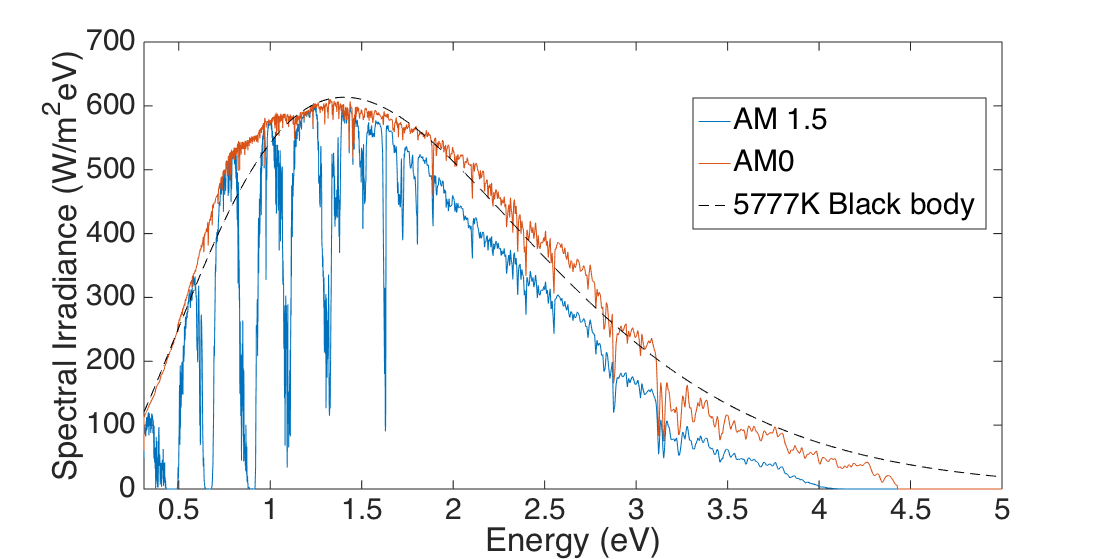
\includegraphics[width=0.75\textwidth]{./Figures/slme/SolarSpectrum.png} 
\caption{\label{fig:slme-solar} Solar Spectra for the extraterrestial AM 0 
(orange) and AM 1.5 (blue) measurements. A black-body spectrum is added as a 
reference point. Data taken from~\cite{International2012}.} 
\end{figure} 
 
\subsection{Absorption}\label{sec:slme-absorption} 
 
When light passes through a semiconductor, a fraction of the photons is 
absorbed by the material, which causes the system to undergo a transition into 
an excited state. An example of such a higher energy state is an electron that 
is excited from the Valence Band (VB) to the Conduction Band (CB). When an 
electron undergoes this transition, it leaves behind a space in the valence 
band for other electrons to move into. Rather than keeping track of the 
valence band electrons, the movement of the empty space is usually represented 
by a positively charged particle, referred to as a \textit{hole}. In this 
framework, the absorption of light is considered as the creation of an 
electron-hole pair, called an \textit{exciton}, through the annihilation of an 
incoming photon. Once the electron-hole pair is no longer bound, they become 
free charge carriers that can move through the semiconductor. 
 
\begin{wrapfigure}{r}{0.5\textwidth}  
\captionsetup{width=0.7\textwidth} 
\centering 
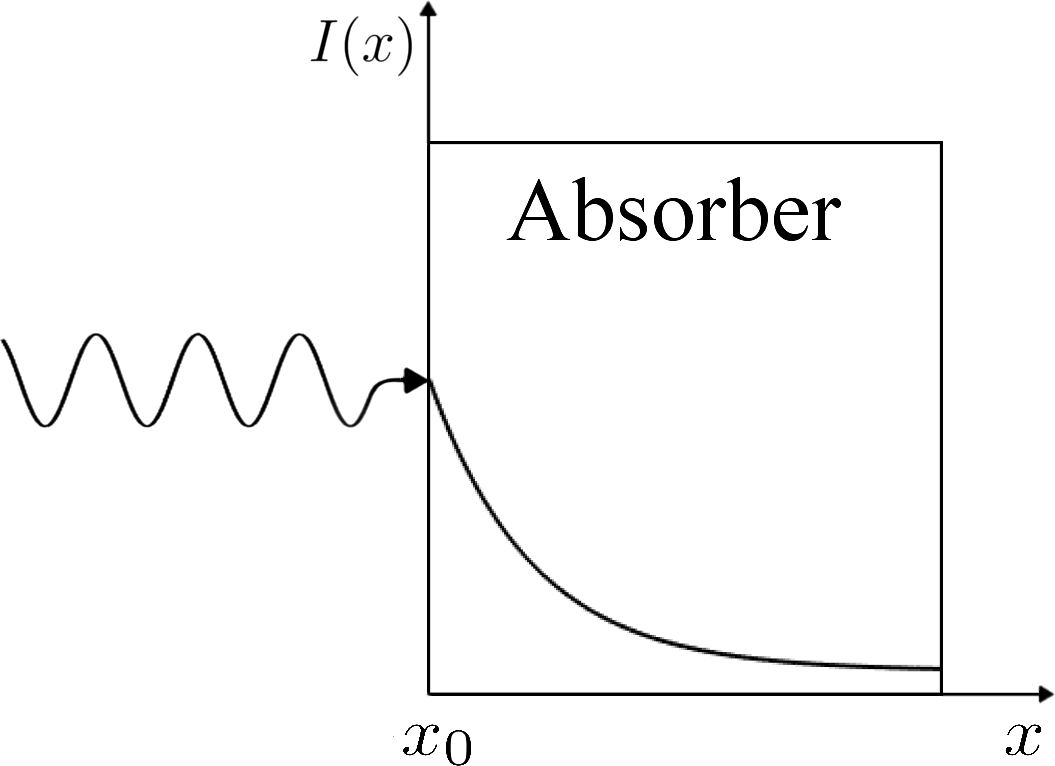
\includegraphics[width=0.48\textwidth]{./Figures/slme/Intensity.png} 
\caption{\label{fig:slme-intensity} Attenuation of the incoming light.} 
\end{wrapfigure} 
 
The absorption process is essential for the generation of carriers that 
produce the current in photovoltaic devices. The strength of the absorption of 
a material for photons of energy $E$ is described by the \textit{absorption 
coefficient} $\alpha(E)$, which determines the attenuation of the incoming 
monochromatic light~\cite{Green1981}: 
\begin{equation}\label{slme:eq-intensity} 
I(x) = I(x_0)e^{-\alpha(E) (x - x_0)}, 
\end{equation} 
where $I(x_0)$ is the intensity upon entering the 
semiconductor~(Fig.~\ref{fig:slme-intensity}). The absorption coefficient is 
related to the extinction coefficient $\hat{k}$, which is defined as the 
imaginary part of the complex index of refraction $\hat{n}_c(E)=n(E)-ik(E)$: 
\begin{equation}\label{slme:eq-absorption} 
\alpha (E)= \frac{4 \pi E \cdot k(E)}{h c}, 
\end{equation} 
where $h$ is Planck's constant and $c$ is the speed of light. Both the real 
and imaginary parts of the index of refraction can be calculated from the 
dielectric tensor, see Section~\ref{dft:sec-linear}. 
 
\begin{figure}[!htp]  
\centering 
\begin{subfigure}{0.50\textwidth} 
\centering 
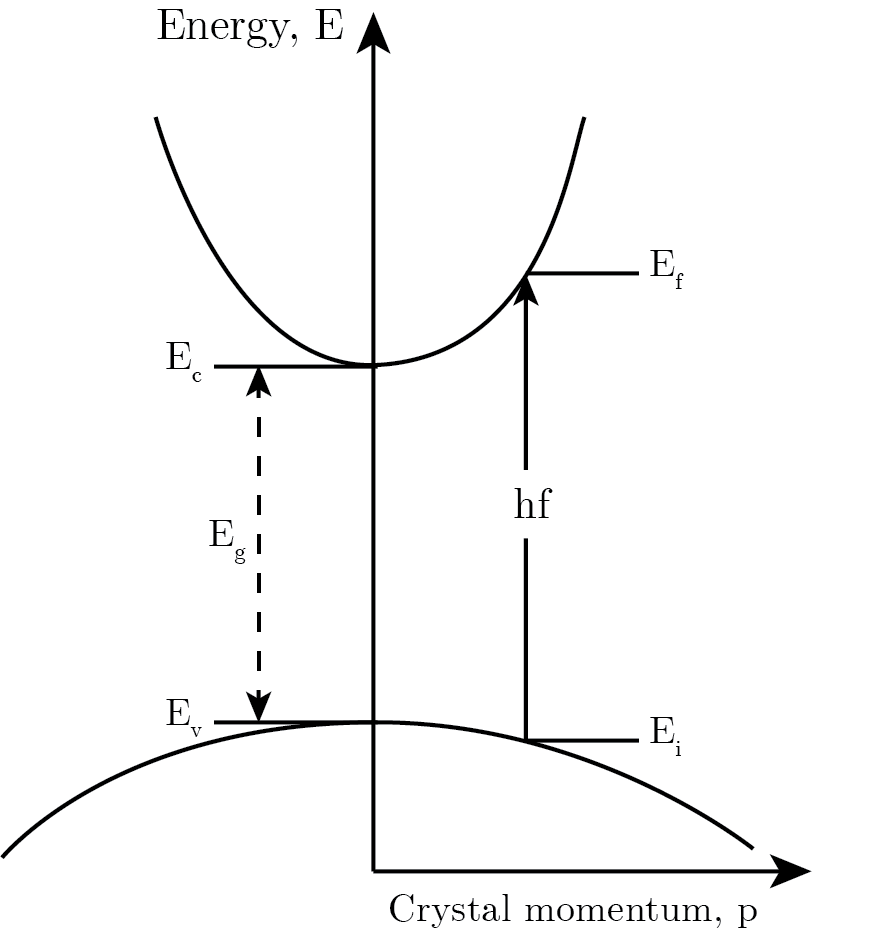
\includegraphics[width=1\linewidth]{./Figures/slme/Direct.png} 
\caption{} 
\end{subfigure}% 
\begin{subfigure}{0.50\textwidth} 
\centering 
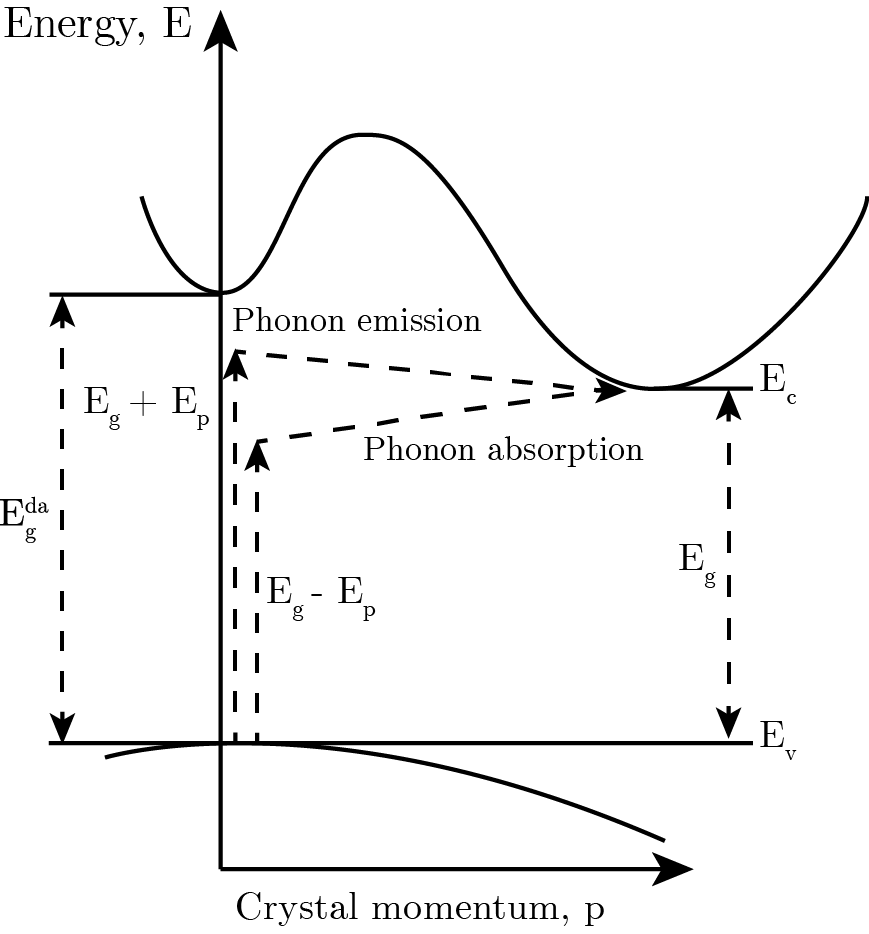
\includegraphics[width=1\linewidth]{./Figures/slme/Indirect.png} 
\caption{} 
\end{subfigure} 
\caption{\label{fig:slme-abstypes}Direct (a) and indirect (b) absorption. 
Adapted from \cite{Green1981}.} 
\end{figure} 
 
An important distinction to make for absorption processes is the difference 
between \textit{direct} and \textit{indirect} transitions 
(Fig.~\ref{fig:slme-abstypes}). When a photon is absorbed to excite an 
electron to a higher energy level, there must be a conservation of energy and 
momentum. For direct transitions, the electron absorbs both the photon energy 
and momentum, the latter of which is very small. However, for indirect band 
gap semiconductors, the minimum energy of the conduction band occurs at a very 
different value of the crystal momentum than the maximum energy of the valence 
band. In this case, absorption of photons with energies around the band gap 
involves the use of phonons, which are quasiparticles describing the 
mechanical vibrations in the crystal, in order to provide the necessary change 
in momentum. For these materials, it is useful to make a distinction between 
the \textit{fundamental} band gap $E_g$ and the \textit{direct allowed} band 
gap $E_g^{da}$, the latter of which is defined as the minimal difference in 
energy of the valence and conduction band at the same crystal momentum. 
 
\subsection{Recombination}\label{sec:slme-recombination} 
 
The electrons that are excited to the conduction band in a semiconductor are 
in a metastable state and eventually return back to the valence band, 
effectively also removing the holes they left after their transition to the 
conduction band. This process is called \textit{recombination}. The lifetime 
of an electron-hole pair depends on the rate of the different recombination 
mechanisms present in the semiconductor material. In this work, we make a 
distinction between three types of recombination: 
 
\begin{enumerate}[] 
 
	\item\textbf{Radiative Recombination} is an interband process that can be 
considered the reverse of the absorption process. An excited electron in the 
conduction band recombines with a hole in the valence band, producing a photon 
which is emitted by the diode~(Fig.~\ref{fig:slme-radrec}). The energy of the 
photon is given by $h \nu = E_c - E_v = E_g$. This recombination mechanism is 
prevalent in direct band gap absorbers such as GaAs, a material used for the 
design of light-emitting diodes~\cite{Green1981}. 
 
\begin{figure}[!htp]  
\centering 
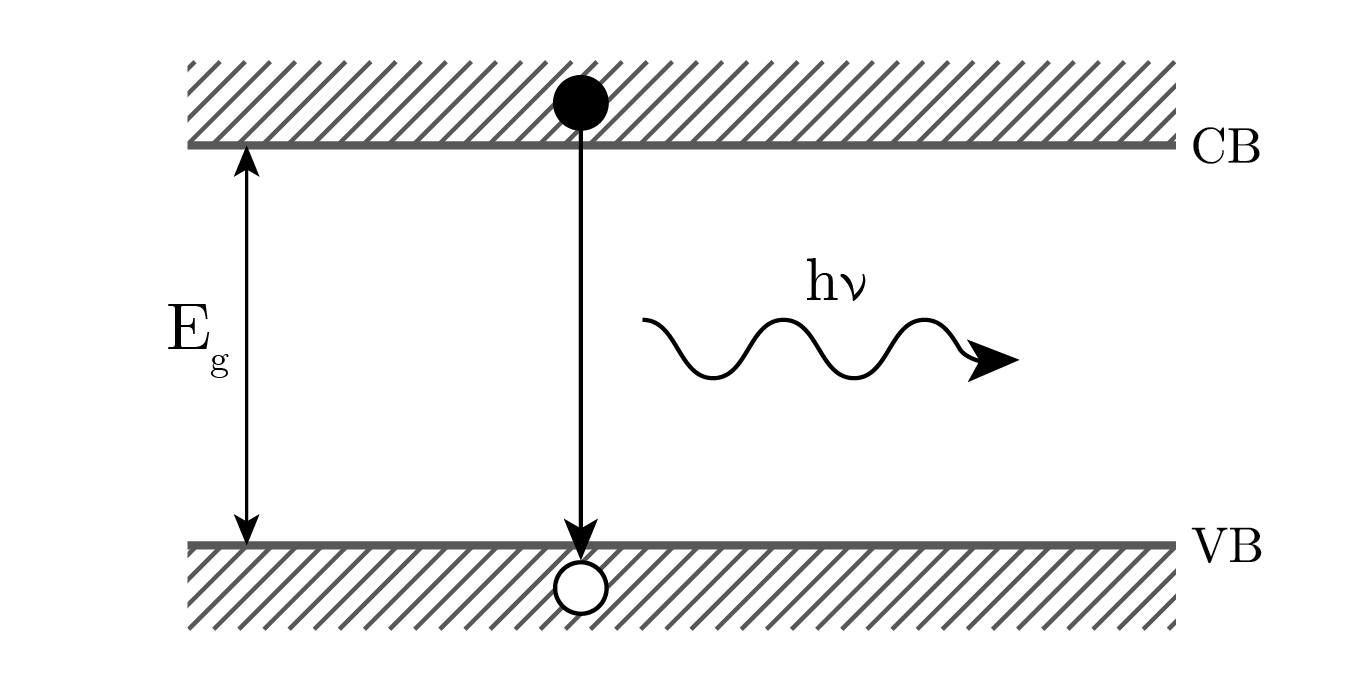
\includegraphics[width=0.65\textwidth]{./Figures/slme/RadRec.png} 
\caption{\label{fig:slme-radrec} Radiative Recombination.} 
\end{figure} 
 
	\item\textbf{Auger Recombination}~\cite{Auger1923} is a three particle 
mechanism, where the energy produced by the electron-hole recombination is 
transferred to another electron (either in the conduction or valence band), 
instead of emitting a photon. The second electron then returns back to its 
original energy via thermal relaxation~(Fig.~\ref{fig:slme-augerrec}). Since 
no light is emitted in this process, it is often referred to as 
\textit{non-radiative} recombination. This type of recombination is dominant 
in indirect band gap materials, of which the most important example is 
silicon~\cite{Nilsson1973}. 
 
\begin{figure}[!htp]  
\centering 
\begin{subfigure}{0.50\textwidth} 
\centering 
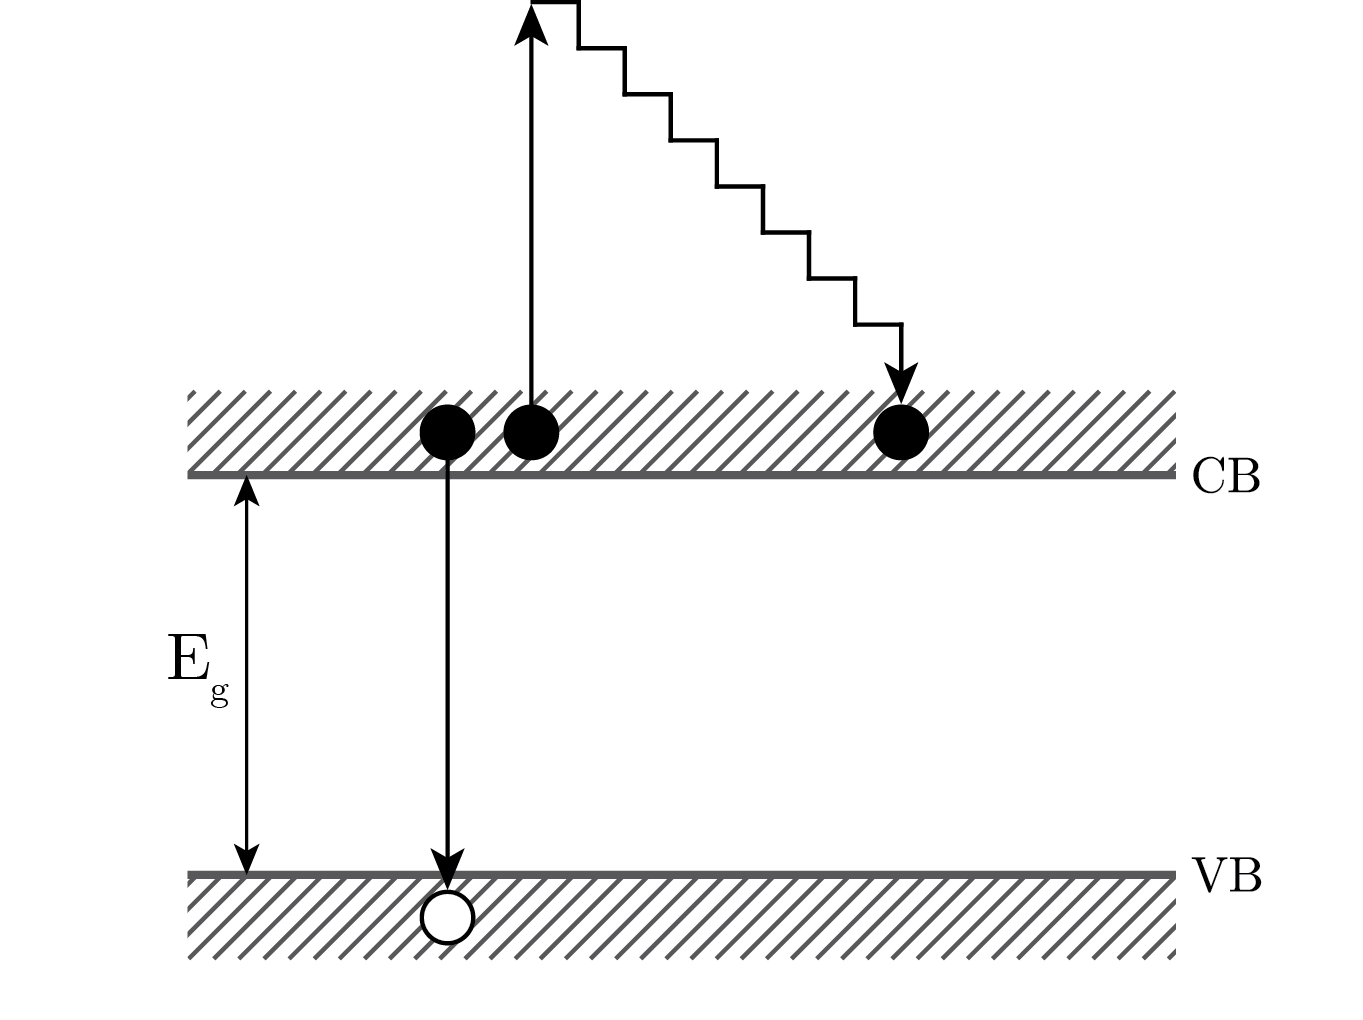
\includegraphics[width=1\linewidth]{./Figures/slme/AugerRec1.png} 
\caption{} 
\end{subfigure}% 
\begin{subfigure}{0.50\textwidth} 
\centering 
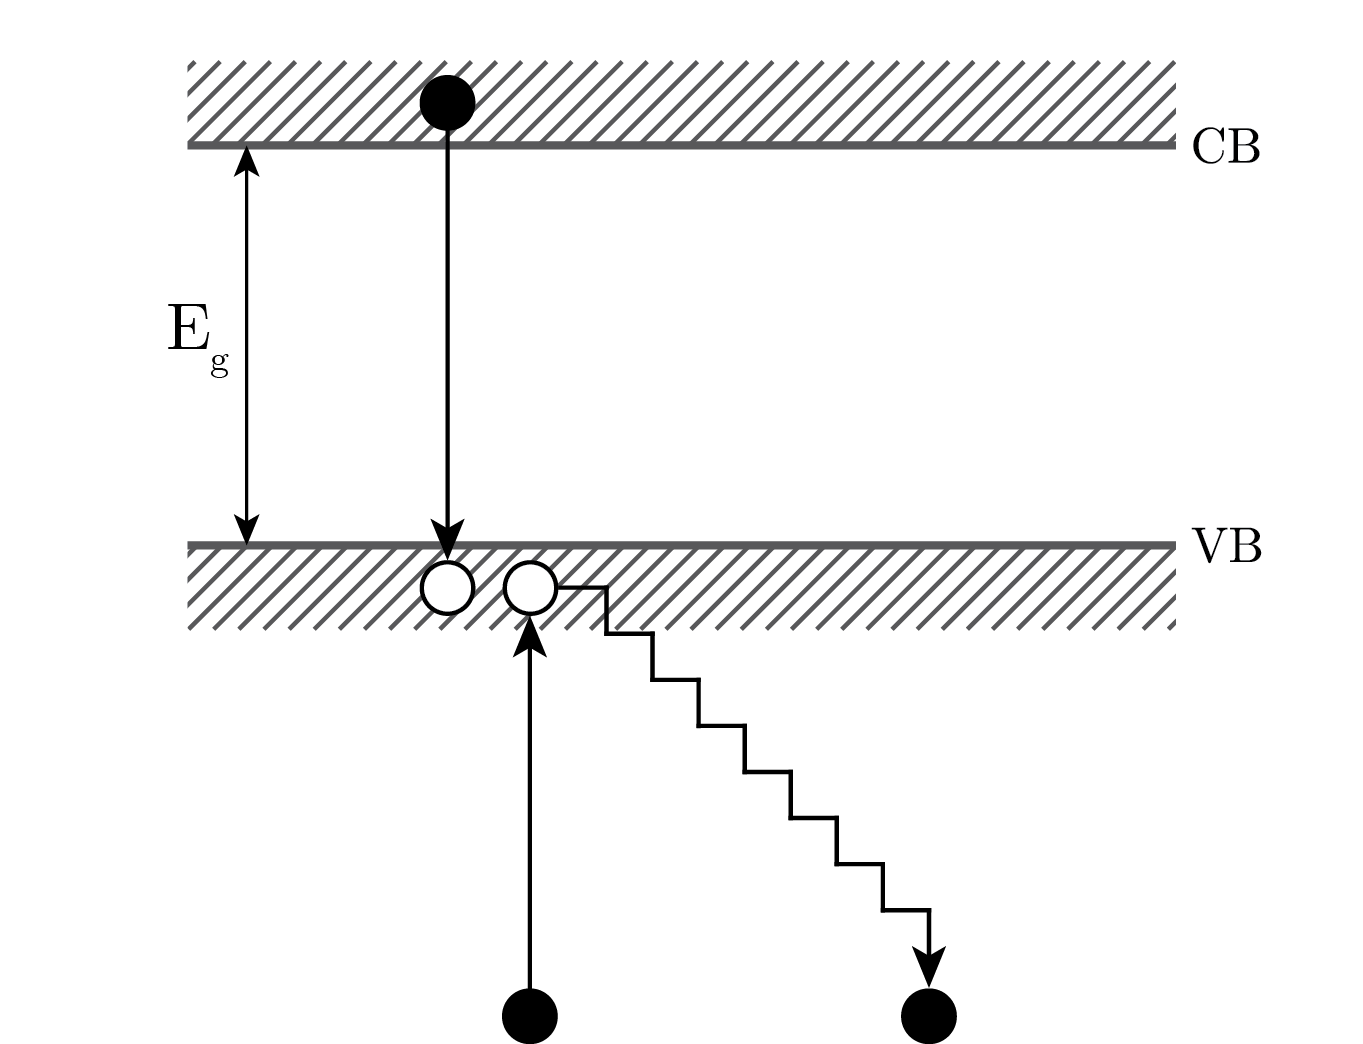
\includegraphics[width=1\linewidth]{./Figures/slme/AugerRec2.png} 
\caption{} 
\end{subfigure} 
\caption{\label{fig:slme-augerrec}Auger Recombination. The recombination 
energy is either passed to an electron in the conduction band (a) or the 
valence band (b).} 
\end{figure} 
 
\vspace{0.2in} 
	\item\textbf{Shockley-Read-Hall Recombination} (SRH) or trap-assisted 
recombination~\cite{Shockley1952}\cite{Hall1952}. This mechanism uses energy 
levels in the band gap, usually produced by defects or impurities, in order to 
relax from the conduction band through a two step process. The electron first 
undergoes a transition to the energy level created by the defect, after which 
it recombines with a hole in the valence band~(Fig.~\ref{fig:slme-SRHrec}). 
Since SRH recombination uses energy levels in the band gap which are produced 
by defects, this mechanism is more important in materials which are heavily 
doped. It is also possible to demonstrate that defect levels situated near the 
middle of the band gap are the most effective for the SRH recombination, 
providing larger recombination rates~\cite{Green1981}. 
 
\begin{figure}[!htp]  
\centering 
\includegraphics[width=0.6\textwidth]{./Figures/slme/SRHrec.png} 
\caption{\label{fig:slme-SRHrec}Shockley-Read-Hall Recombination.} 
\end{figure} 
 
\end{enumerate} 
 
\pagebreak[4] 
\subsection{PN - Junction} 
 
When a semiconductor is doped with impurity atoms that have more valence 
electrons, there are more electrons in the conduction band that can contribute 
to the conductivity of the material. This is called a \textit{n-type} 
semiconductor. If we introduce atoms that have less valence electrons, there 
is an increased amount of holes in the valence band, also creating a better 
conductivity and what is referred to as a \textit{p-type} semiconductor. By 
joining a n-type and p-type semiconductor, we form what is known as a 
\textit{P-N~junction~diode}~\cite{Shockley1949}~(Fig.~\ref{fig:slme-PNjunction}). 
 
\begin{wrapfigure}{r}{0.55\textwidth} 
\centering 
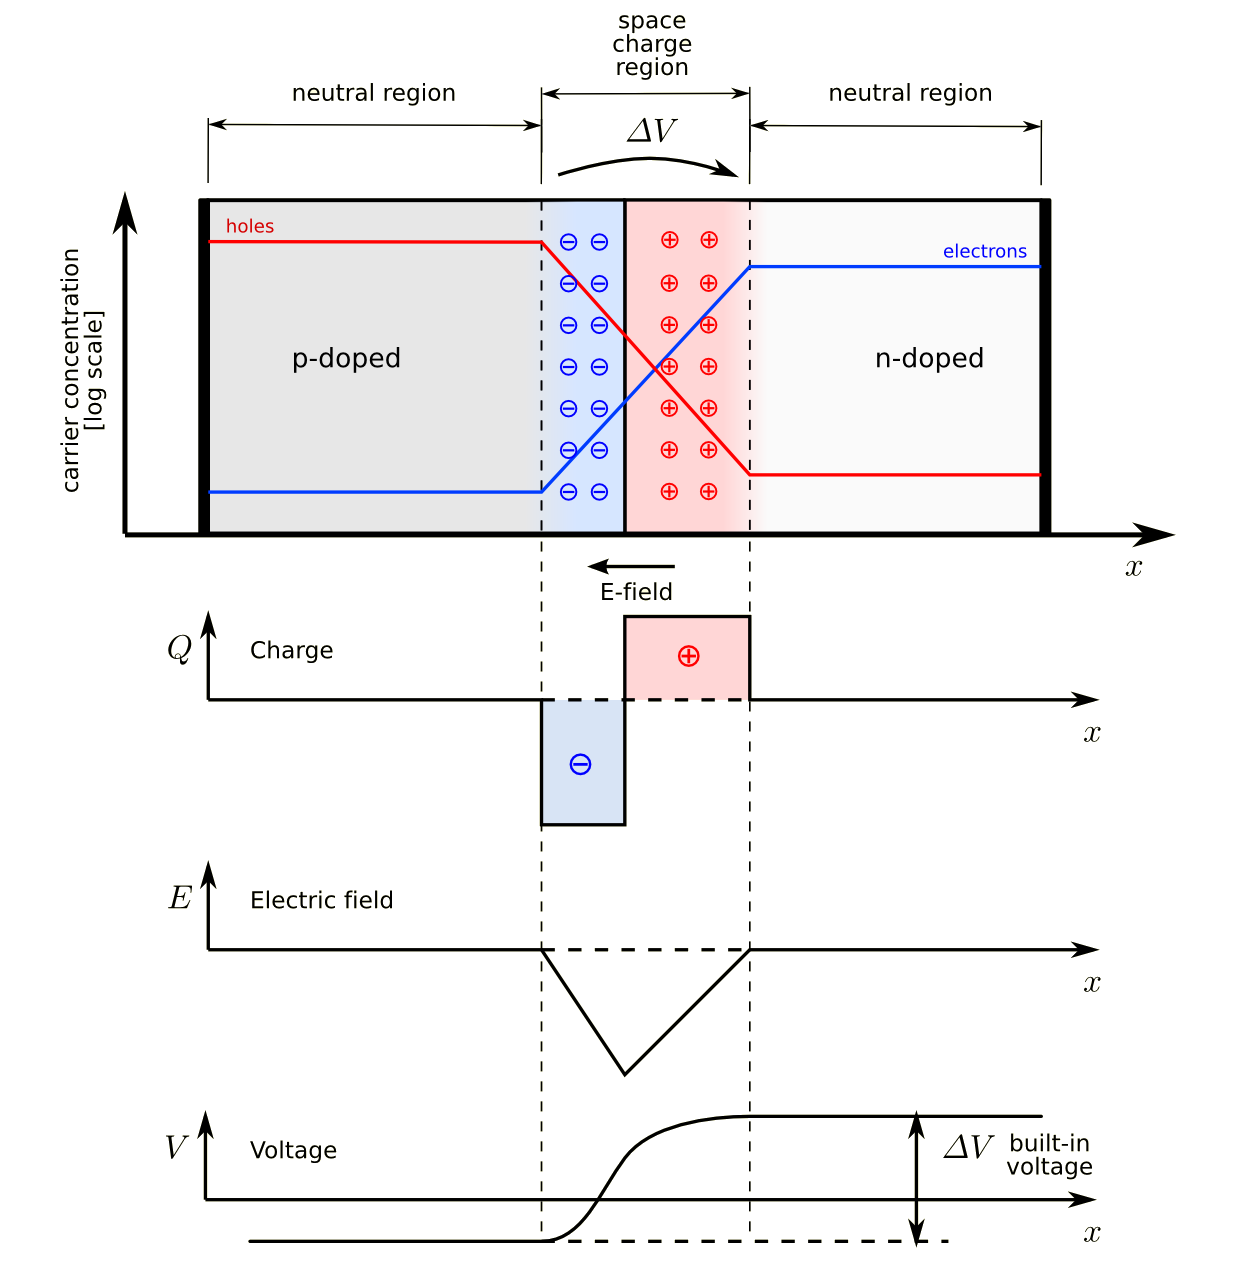
\includegraphics[width=0.5\textwidth]{./Figures/slme/PN-Junction.png} 
\caption{\label{fig:slme-PNjunction} The P-N Junction. \cite{wikigraph}} 
\end{wrapfigure} 
 
An important effect caused by putting these two types of materials together is 
the creation a \textit{depletion region}, which is a result of the electrons 
and holes looking for an equilibrium by moving to the other side of the P-N 
junction. When the electrons move from the n-type to the p-type region, they 
leave behind positively charged ion cores. Similarly, holes moving across the 
junction create a negative surplus charge in the p-type semiconductor. This 
charge imbalance creates an electric field at the center region of the diode, 
which eventually puts a stop to the migration of electrons and holes. The 
result is a potential difference across the P-N junction, which is required to 
separate the charge carriers generated by the absorption of incoming light. 
 
By applying a voltage across the P-N junction, we can influence the strength 
of the electric field in the depletion region. Under \textit{forward bias}, we 
decrease the voltage difference over the diode, making it easier for the 
charge carriers to move across the junction. This has the potential of 
increasing the power output, but also raises the possibility that the 
electrons and holes can recombine. In the \textit{reverse} bias case, the 
electric field across the junction is lowered, and the charge carriers are 
more or less confined to their respective regions.  
 
\subsection{Ideal Diode Law} 
 
In order to properly model the functioning of a solar cell, we need to know 
the I-V characteristic of the P-N~junction. If we write down the electron and 
hole densities as $n(x)$ and $p(x)$, along with their respective current 
densities $J$, mobilities $\mu$ and diffusivity constants $D$, the dynamics of 
the electrons and holes in the different regions of the P-N diode can be 
characterized by a set of basic equations~\cite{Shockley1949}: 
\vspace{0.1in} 
\begin{enumerate} 
\item \textbf{Poisson's Equation: } \begin{equation}\frac{\partial 
E_x}{\partial x} = \frac{\rho}{\epsilon},\end{equation} 
 
\item \textbf{Transport Equations: } \begin{equation}J_n = e \mu_n n(x) E_x + 
e D_n\frac{\partial n }{\partial x}, \hspace{0.6in} J_p = e \mu_p p(x) E_x - e 
D_p \frac{\partial p}{\partial x},\end{equation} 
 
\item \textbf{Continuity Equations: } \begin{equation}\frac{\partial 
n}{\partial t} = \frac{1}{e} \frac{\partial J_n}{\partial x} - (U - G), 
\hspace{0.6in} \frac{\partial p}{\partial t} = - \frac{1}{e} \frac{\partial 
J_p}{\partial x} - (U - G),\end{equation} 
 
\end{enumerate} 
where $E_x$ is the electric field, $\rho$ is the charge density, $\epsilon$ is 
the material permittivity and $e = 1.602\cdot 10^{-19}$ C is the standard 
electronic charge. The generation rate $G$ and recombination rate $U$ describe 
the creation and annihilation of electron-hole pairs, and are determined by 
the absorption and recombination processes described in 
Sections~\ref{sec:slme-absorption} and~\ref{sec:slme-recombination}.  
 
These equations can be readily solved using numerical approaches. However, by 
applying a few approximations, it is possible to derive a general relation for 
the I-V characteristic of a P-N~junction, known as the \textit{Ideal Diode 
Law}~\cite{Shockley1949}: 
\begin{equation}\label{eq:slme-idealdiode} 
I = I_0 (e^\frac{e V}{k_B T} - 1), 
\end{equation} 
with $k_B$ Boltzmann's constant and $T$ the temperature of the diode. The 
current $I_0$ in Eq.~\ref{eq:slme-idealdiode} is called the \textit{reverse 
saturation} current, which is a measure of the recombination in the device. In 
light of its connection with recombination effects, $I_0$ is also referred to 
as the recombination current~\cite{Cuevas2014}. 
 
\subsection{Working Principles of a Solar Cell} 
 
We now turn to a basic discussion of the working principles of photovoltaic 
devices~\cite{Fonash2010}. Figure~\ref{fig:slme-solarcell} shows the design of 
a conventional solar cell. The top and base layer usually consist of a n-type 
and p-type doped material, not necessarily derived from the same compound. The 
layers form a P-N junction, which is connected on both sides to electrodes 
that are responsible for extracting the charge carriers from the photovoltaic 
device. In order to prevent losing too much of the incoming light to 
reflection, an \textit{Anti-Reflective} (AR) coating~\cite{Swatowska2011} is 
applied to the top layer. Many solar cells also use a reflective back surface 
(not shown in figure) to increase the path length of the incoming light 
through the absorber layer. 
 
\begin{figure}[!htp]  
\centering 
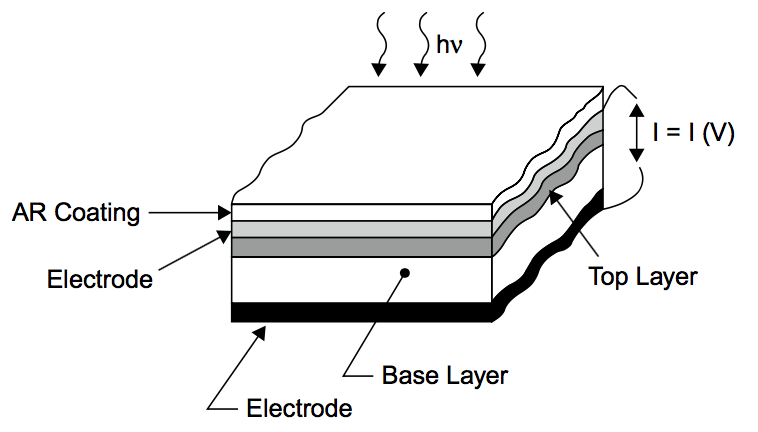
\includegraphics[width=0.8\textwidth]{./Figures/slme/structure.png} 
\caption{\label{fig:slme-solarcell} Cross section of a typical solar cell. 
Taken from~\cite{Fonash2010}.} 
\end{figure} 
 When the absorber layer captures an incoming photon, the material is brought 
into a higher energy state, usually by the creation of an exciton or free 
electron-hole pair. In the case an exciton is produced, it must first be 
dissociated into an electron and a hole. Once the charge carriers are free to 
move, they go to their respective electrode interface. During this stage it is 
crucial that the electron does not recombine with another hole before it is 
extracted from the device. Once the electron reaches the cathode, it makes its 
way to an external load, where it transfers its energy before moving to the 
anode. Finally, the electron reaches the bottom layer and recombines with a 
hole. 
 
\pagebreak[4] 
 
The process of generating a current from a solar cell can be summarized in 
five steps, which are visualized by drawing an energy band diagram for the 
absorption process in Figure~\ref{fig:slme-working}: 
 
\vspace{0.25in} 
\begin{enumerate}[I.]  
 
\item Transition into an excited state by the absorption of an incoming 
photon.  
 
\item Conversion of the excited state into at least one electron-hole pair. 
 
\item Transport of the charge carriers to their respective electrodes. 
 
\item Transfer of the electron's energy at an exterior load. 
 
\item Recombination of the electron with the hole. 
 
\end{enumerate} 
\vspace{0.50in} 
 
\begin{figure}[!htp]  
\centering 
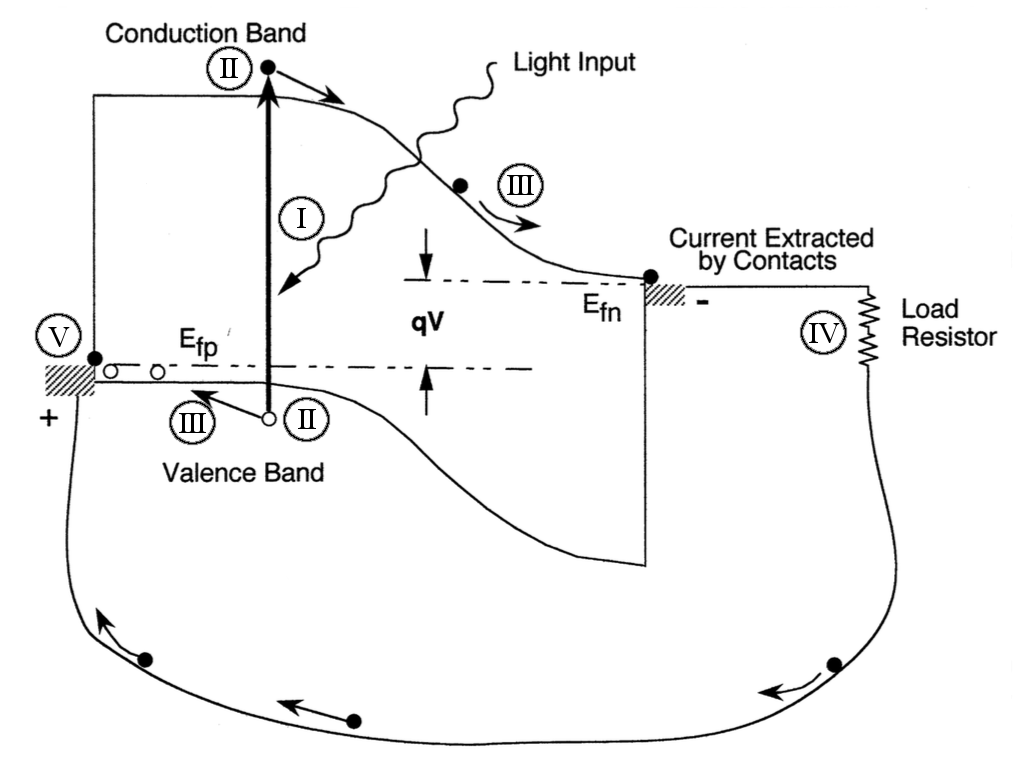
\includegraphics[width=0.9\textwidth]{./Figures/slme/Working.png} 
\caption{\label{fig:slme-working} Step by step visualisation of the different 
processes in a solar cell. Adapted from \cite{Smestad2002}.} 
\end{figure} 
 
\pagebreak[4] 
 
The I-V characteristic of the solar cell under dark conditions is given by the 
ideal diode law~(Eq.~(\ref{eq:slme-idealdiode})). When the solar cell is 
illuminated, the I-V equation becomes\footnote{Note that in principle, the I-V 
curve is given by $I = I_0 (e^\frac{e V}{k_B T} - 1) - I_{sc}$, but the 
convention is to invert the current axis.}~\cite{Lindholm1979}: 
\begin{equation}\label{eq:slme-V} 
I = I_{sc} - I_0 (e^\frac{e V}{k_B T} - 1), 
\end{equation} 
where $I_{sc}$ is the \textit{short circuit} current. This current is a result 
of the generation of charge carriers due to absorption of incoming photons. In 
many cases, the currents in Eq.~\ref{eq:slme-IV} are expressed as current 
densities\footnote{Note that these current densities are not defined in the 
conventional way. Rather, they are considered as currents per surface area of 
the solar cell. This allows us to ignore the surface area of the solar cell in 
our discussion.} ($J,J_0,J_{sc}$), and we follow a the same convention 
throughout this text. Figure~\ref{fig:slme-IV_char}(a) shows the I-V 
characteristic of a solar cell under illuminated and dark conditions, whereas 
Figure~\ref{fig:slme-IV_char}(b) demonstrates the definition of the 
\textit{Fill Factor}~(FF)~\cite{Fonash2010}: 
\begin{equation} 
FF = \frac{P_{m}}{V_{oc} J_{sc}}, 
\end{equation} 
where $P_m = J_m V_m$ is the maximum power density and $V_{oc}$ is the 
\textit{open circuit} voltage, which is the voltage of the diode at $J = 0$: 
\begin{equation} 
J_{sc} - J_0 (e^\frac{eV_{oc}}{k_B T}-1) = 0 \hspace{0.1in} \Leftrightarrow 
\hspace{0.1in} V_{oc} = \frac{k_B T}{q} \ln (\frac{J_{sc}}{J_0} + 1). 
\end{equation} 
The fill factor is a measure for how close a given characteristic is to 
obtaining the ideal power density $J_{sc}V_{oc}$, i.e. operating at the 
short-circuit current and open-circuit voltage. 
 
\begin{figure}[h]  
\centering 
\begin{subfigure}{0.5\textwidth} 
\centering 
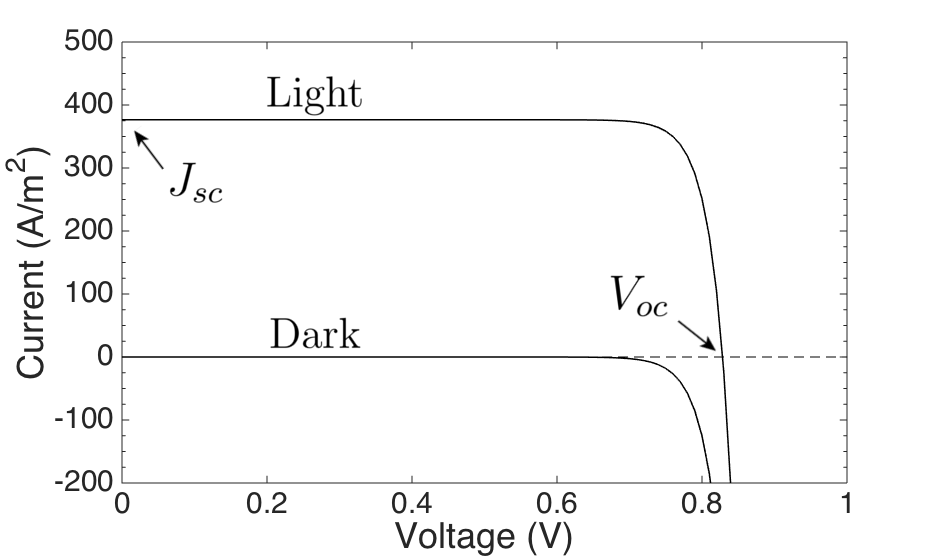
\includegraphics[width=1\linewidth]{./Figures/slme/IVchar.png} 
\caption{} 
\end{subfigure}% 
\begin{subfigure}{0.5\textwidth} 
\centering 
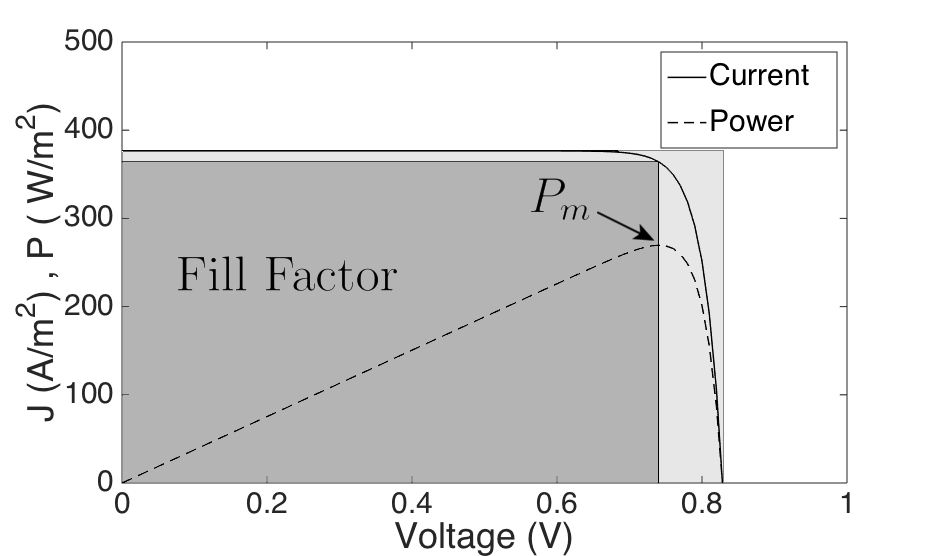
\includegraphics[width=1\linewidth]{./Figures/slme/FillFactor.png} 
\caption{} 
\end{subfigure} 
\caption{\label{fig:slme-IV_char} (a) I-V curve of a solar cell under dark and 
illuminated (light) conditions. (b) Power maximization and the corresponding 
fill factor, given by the dark area ($P_m$) divided by the light area ($V_{oc} 
J_{sc}$).} 
\end{figure} 
 
\section{Selection Metric}\label{sec:slme-metric} 
 
Materials play a central role in the effort to produce cheaper and more 
efficient solar cells. The discovery of improved absorber materials has the 
potential to significantly increase the cost-effectiveness of photovoltaic 
devices, but experimental trial and error methods are often slow and 
expensive. Currently, we know the properties of less than 1\% of all 
materials, and it can require decades to identify new compounds for a 
technological application~\cite{Jain2013}. This process needs to be more 
efficient, by reducing both the time and cost of material development. Here, 
computational material modeling can provide a valuable assist to the material 
design process, by screening groups of materials for those that have the best 
properties.  
 
Over the past few decades, there has been a significant increase in the 
capability of high performance computing, which shows no signs of abating. 
Computer simulations that use sophisticated quantum models have the power to 
analyze many properties of materials, offering a relatively cheap and 
effective method to discover new potential candidates for solar cell absorber 
layers. Recently developed \textit{High Throughput} 
methods~\cite{Curtarolo2013}~\cite{Sarmadian2016} provide an automated 
procedure to screen large amounts of compounds. The combination of these 
rapidly evolving techniques with a suitable selection metric has the potential 
of identifying the most promising materials from many different possible 
structures. The \textit{Spectroscopic Limited Maximum Efficiency} (SLME) is a 
calculable selection metric that tries to improve upon its predecessors by 
including the absorption spectrum, calculated from first-principles methods, 
in its estimation of the efficiency of materials as absorber layers. This 
section is dedicated to explaining the SLME metric, as well as its 
predecessor, the Shockley-Queisser (SQ) limit.  
 
\subsection{Solar Cell Efficiency} \label{slme:sec-efficiency} 
 
In order to compare the performance of solar cells, we need to have a gauge 
for their efficiency. A sensible way of defining the efficiency of a 
photovoltaic device is as the ratio of the maximum power density $P_m$, 
produced by the solar cell, and the total incident power density from the 
solar spectrum~\cite{Fonash2010}: 
\begin{equation} 
\eta = \frac{P_m}{P_{in}}. 
\end{equation} 
When measuring the efficiency, it is important to use agreed upon conditions 
for the calculation of both power densities. For the solar spectrum, 
researchers normalize the AM1.5G spectrum to produce a total incident power 
density of 1 \si{\watt \per \meter\square}, and generate it in a lab to find 
experimental values for the output power density of the solar cell. The 
reference temperature of the device is usually 25 \si{\celsius}. 
Figure~\ref{fig:slme-effchart} shows the evolution of the maximum efficiency 
found for different types of solar cells. We can see that the current highest 
performance is achieved by the multijunction PV devices, which use a 
combination of P-N junctions with a different band gap for each semiconductor 
compound~\cite{Dimroth2007}. The materials are chosen with decreasing band 
gaps, so that the higher energy photons are absorbed first. In this way, the 
multijunction solar cell absorbs photons over a large range of frequencies, 
and loses less energy to thermic relaxation of electrons in the conduction 
band. Other promising results are shown for the \textit{thin film} 
technologies~\cite{Shah2004}, which focus on reducing the material consumption 
in an attempt to make PV energy generation more financially competitive. 
Finally, there is an increasing interest in developing organic cells, which 
have the potential of being very cost effective and having far less impact on 
the environment. 
 
\begin{figure}[!htp]  
\centering 
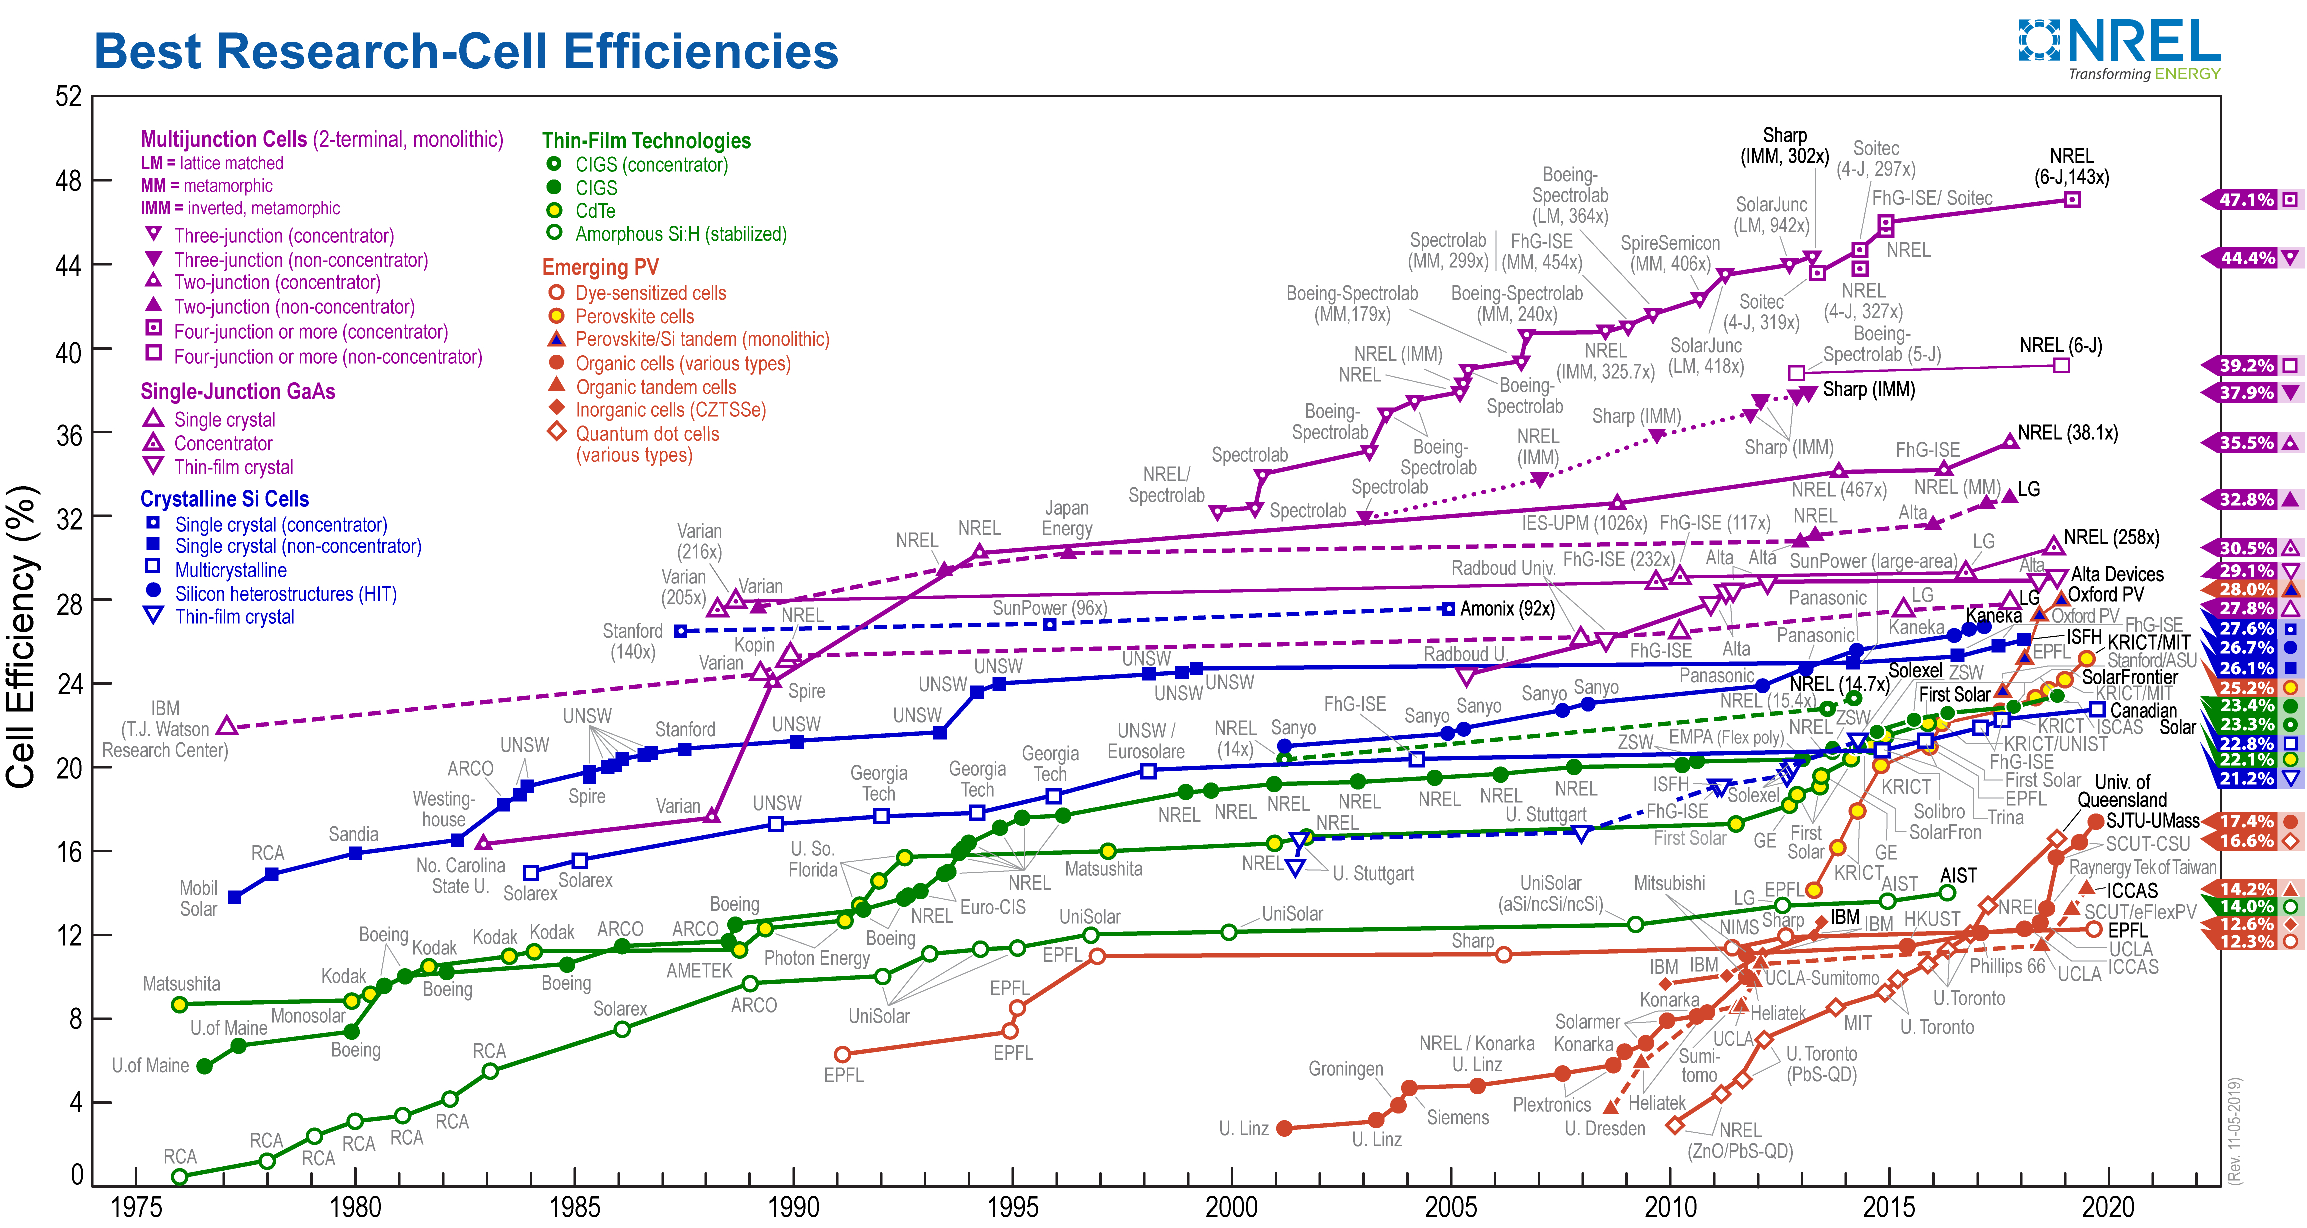
\includegraphics[width=1\textwidth]{./Figures/slme/efficiency_chart.png} 
\caption{\label{fig:slme-effchart} Overview of the evolution of solar cell 
efficiencies over the past four decades. Provided by NREL~[CITE].} 
\end{figure} 
 
\subsection{Shockley-Queisser Limit} \label{sec:slme-SQlimit} 
 
In 1961, Shockley and Queisser proposed a theoretical upper limit for the 
efficiency of PV devices with a single P-N junction, which solely depends on 
the band gap of the absorber material~\cite{Shockley1949}. Their derivation is 
based on the principle of \textit{detailed balance}, which states 
that~\cite{Klein1955}: ``\textit{transitions between any two states take place 
with equal frequency in either direction at equilibrium}". They also make the 
assumption that every incident photon with an energy above the band gap ($h\nu 
> E_g$), no matter how high its energy, produces a single electron-hole 
pair\footnote{As Shockley and Queisser note in their original paper, it is 
possible to have a higher absorber layer efficiency than the SQ limit, for 
example if we include the possibility that one photon produces multiple 
electron-hole pairs.}. This corresponds to setting the absorptivity $a(E)$ - 
the chance that an incoming photon is captured by the absorber layer - to a 
step function: 
\begin{equation}\label{eq:slme-step_a} 
a(E) =  \begin{cases} 0, & \mbox{if } E < E_g \\ 1, & \mbox{if } E \geq E_g 
\end{cases} 
\end{equation} 
 
To calculate $P_m$, the power density $P = JV$ is maximized versus the voltage 
$V$, where the current density $J$ is derived from the ideal $J-V$ 
characteristic of an illuminated solar cell (Eq.~(\ref{eq:slme-V})): 
\begin{equation}\label{eq:slme-JV} 
J = J_{sc} - J_0 \left(e^{\frac{eV}{k_B T}} - 1\right). 
\end{equation} 
The short-circuit current density $J_{sc}$, also known as the photogenerated 
current or the illuminated current, is calculated from the number of photons 
of the solar spectrum that are absorbed by the solar cell: 
\begin{align} 
J_{sc} = e &\int_0^{\infty} a(E) \Phi_s (E) dE \\ 
\stackrel{(\ref{eq:slme-step_a})}{=} e &\int_{E_g}^{\infty} \Phi_s (E) dE 
\label{eq:slme-Ish} 
\end{align} 
where $\Phi_s(E)$ is the photon flux density of the solar spectrum. In their 
original paper, Shockley and Queisser used a blackbody spectrum of $T_s = 
6000~\si{\kelvin}$, but the current convention is to use the AM1.5G solar 
spectrum~\cite{International2012}.  The reverse saturation current density 
$J_0$ is calculated by considering the principle of detailed balance, i.e. in 
equilibrium conditions the rate of photon emission from radiative 
recombination must be equal to the photon absorption from the surrounding 
medium. Because the cell is considered to be attached to an ideal heat sink, 
the ambient temperature is the same as that of the solar cell. Hence, the 
spectrum of the surrounding medium is that of a black body at cell temperature 
$T$: 
\begin{align} 
J_0 = e \pi &\int_0^{\infty} a(E) \Phi_{bb}(E) dE\nonumber \\ 
= e \pi &\int_0^{\infty} a(E) \frac{2E^2}{h^3 c^2} \frac{dE}{e^{\frac{E}{k_B 
T}}-1} \\ 
\stackrel{(\ref{eq:slme-step_a})}{=} e \pi &\int_{E_g}^{\infty} 
\frac{2E^2}{h^3 c^2} \frac{dE}{e^{\frac{E}{k_B T}}-1} \label{eq:slme-I0} 
\end{align} 
where $h$ is Planck's constant and $c$ is the speed of light. Because of its 
connection with the recombination of electron-hole pairs at equilibrium, $J_0$ 
is also referred to as the recombination current density~\cite{Cuevas2014}. 
This is the convention we will use here. 
 
The resulting function for the efficiency only depends on the band gap $E_g$ 
and is called the Shockley-Queisser or detailed balance limit. 
Figure~\ref{fig:slme-SQlimit} shows the curve for the SQ limit for band gaps 
with an efficiency above 5\%. The maximum conversion of the incoming power 
density is 33.7\%, found for a band gap of 1.34 eV. 
 
\begin{figure}[!htp]  
\centering 
\includegraphics[width=0.7\textwidth]{./Figures/slme/SQlimit.png} 
\caption{\label{fig:slme-SQlimit} The Shockley-Queisser limit, based on the 
AM1.5G spectrum.} 
\end{figure} 
 
% Double code // compare and keep whatever is better 
% 
%Once we have acquired the dielectric function, we can calculate the 
absorption coefficient 
%\begin{equation} 
%	\alpha(E) = \frac{4 \pi E }{hc}\hat{k}(E), 
%\end{equation} 
%with $h$ Planck's constant and $c$ the speed of light, from the extinction 
coefficient $\hat{k}(E)$: 
%\begin{equation} 
%	\hat{k}(E) = \sqrt{\frac{|\varepsilon(E)| - \varepsilon^{(1)}(E)}{2}}. 
%\end{equation} 
%This allows us to determine the absorptivity $a(E) = 1 - e^{-2\alpha(E)L}$ 
for an absorber layer of thickness $L$ with a reflecting back 
surface~\cite{Green1981}.  
% 
%The theoretical maximum solar cell efficiency is defined as 
%\begin{equation}\label{eq:efficiency} 
%\eta = \frac{P_m}{P_{in}}, 
%\end{equation} 
%where $P_m$ is the maximum power density and $P_{in}$ is the total incident 
power density from the solar spectrum. For the SLME, the maximum power density 
is derived using the $J$-$V$ characteristic of the solar cell: 
%\begin{equation}\label{eq:power} 
%		P = J V =  \left( J_{sc} - J_0 \left(e^{\frac{eV}{kT}} - 1 \right) \right) 
V, 
%\end{equation} 
%with $J$ the total current density, $V$ the potential over the absorber 
layer, $k$ Boltzmann's constant, $T$ the temperature of the device and $e$ the 
elementary charge. The short circuit current density $J_{sc}$ and the reverse 
saturation current density $J_0$ are calculated from the absorptivity $a(E)$ 
of the material, as well as the AM1.5G solar spectrum $I_{sun}(E)$ and the 
black-body spectrum $I_{bb}(E,T)$: 
%\begin{equation}\label{eq:currents} 
%\begin{aligned} 
%J_{sc} &= e \int_0^\infty a(E) I_{sun} (E) dE, 
%\\ J_0 &= \frac{J_0^r}{f_r} = \frac{e\pi}{f}\int_0^\infty a(E)I_{bb}(E,T)dE, 
%\end{aligned} 
%\end{equation} 
%where $J_0^r$ is the radiative recombination current density. The fraction of 
radiative recombination $f_r$ is modeled using a Boltzmann factor: 
%\begin{equation}\label{eq:fraction} 
%	f_r = \exp\left({\dfrac{E_g^{da}-E_g}{kT}}\right), 
%\end{equation} 
%where $E_g$ and $E_g^{da}$ are respectively the fundamental and direct 
allowed band gap.  
 
%Note that in the original expressions, Shockley and Queisser also included a 
geometrical factor. However, because we assume the solar cell to have a 
perfect antireflective coating, as well as a reflective back surface, the 
geometrical factor is equal to unity~\cite{Ruhle2016}. 
 
 
\subsection{Spectroscopic Limited Maximum Efficiency} \label{sec:slme-SLME} 
 
Although the work of Shockley and Queisser was an important step forward, only 
relying on the band gap as the only piece of information to determine the 
efficiency of a compound is too limited. Modern quantum mechanical models 
allow us to determine the response of a material to an incident photon in much 
more detail, based on data derived from first-principles calculations. The 
Spectroscopic Limited Maximum Efficiency, introduced by Yu and 
Zunger~\cite{Yu2012}, attempts to use these advances in computational science 
to get a better picture of which semiconductors have the greatest potential as 
absorber materials. The SLME also includes the thickness of the absorber layer 
in the calculation of the maximum efficiency, and is therefore particularly 
suited to study the thin-film technologies presented in 
Figure~\ref{fig:slme-effchart}. Since its conception, the SLME has been 
successfully applied to perovskites~\cite{Yin2014, Yin2015, Yin2015b, 
Meng2016}, chalcogenides~\cite{Hong2016, Sarmadian2016}, direct band gap 
silicon crystals~\cite{Lee2014, Oh2015} and other materials~\cite{Yu2012b, 
Yokoyama2013, Heo2014, Huang2015}.  
 
The SLME tries to improve upon the Shockley-Queisser limit in two ways:  
\vspace{0.1in} 
\begin{enumerate}[I.] 
 
\item Instead of assuming that every photon with an energy greater than the 
band gap is absorbed with absolute certainty, the SLME incorporates the 
absorption coefficient $\alpha(E)$ (Sec.~\ref{sec:slme-absorption}) of the 
material in order to more accurately model the generation of electron-hole 
pairs. After calculating the absorption coefficient from first-principles, we 
include it in both the calculation of the short circuit current and the 
recombination current. This is done through the \textit{absorptivity} $a(E)$, 
which is defined as the fraction of sunlight that is absorbed when the photons 
pass twice through a layer of thickness $L$: 
\begin{equation} \label{eq:slme-absorptivity} 
a(E) = 1 - e^{-2 \alpha(E) L}. 
\end{equation} 
 
\item The SLME models radiative recombination using the absorptivity in 
combination with the black-body spectrum at the temperature $T$ of the device. 
In order to include the non-radiative recombination mechanisms, Yu and Zunger 
make the following consideration. The total reverse saturation current is the 
sum of the radiative and non-radiative parts $J_0 = J_0^r + J_0^{nr}$. If one 
defines $f_r$ as the fraction of radiative recombination\footnote{Actually, 
Shockley and Queisser also considered the fraction of radiative recombination 
in their approach. They did not, however, provide a model to calculate it, 
simply observing that the maximum efficiency is significantly reduced for 
small fractions $f_r$.}, the total reverse saturation current density can be 
written as: 
\begin{equation} 
J_0^r = f_r J_0 \hspace{0.1in} \Leftrightarrow \hspace{0.1in} J_0 = 
\frac{J_0^r}{f_r}. 
\end{equation} 
The fraction of radiative recombination is expressed as a Boltzmann factor:  
\begin{equation} \label{eq:slme-fraction} 
f_r = e^{-\frac{\Delta}{kT}}, 
\end{equation} 
where $\Delta$ is the difference in energy between the direct allowed and 
fundamental band gap: $\Delta = E_g^{da} - E_g$. Using this approximation, the 
recombination of direct band gap absorber materials is entirely radiative in 
nature ($f_r = 1$). However, for indirect band gap semiconductors ($\Delta 
\neq 0$), the non-radiative recombination quickly becomes the dominant 
mechanism. This is in accordance with what is observed experimentally for 
direct and indirect band gap semiconductors. 
\end{enumerate} 
\vspace{0.1in} 
 
When determining the SLME in practice, we start by calculating the 
absorptivity from the absorption coefficient, derived from the ab initio 
methods. Once we know the absorptivity, we use it to determine the short 
circuit and radiative reverse saturation current densities: 
\begin{equation} \label{eq:slme-currents} 
\begin{aligned} 
J_{sc} &= e \int_0^\infty a(E)  \Phi_{sun} (E) dE, 
\\ J_0^r &= e\pi \int_0^\infty a(E)  \Phi_{bb} (E,T) dE, 
\end{aligned} 
\end{equation} 
where $I_{sun}(E)$ and $I_{bb}(E,T)$ are once again the solar spectrum AM1.5G  
and the black-body spectrum at device temperature $T$. We then use the optical 
and fundamental band gap, also retrieved from first-principles calculations, 
to derive the radiative fraction $f_r$ (Eq.~(\ref{eq:slme-fraction})). From 
here, it is a simple matter of dividing $J_0^r$ by $f_r$ to find the total 
recombination current density $J_0$. Once we know both $J_{sc}$ and $J_0$, we 
use the $J$-$V$ characteristic of the illuminated P-N junction 
(Eq.~(\ref{eq:slme-JV})) to calculate the total current density versus a range 
of voltages $V$ up to the open circuit voltage $V_{oc}$. Finally, we maximize 
the product $J\cdot V$ versus $V$ to find the maximum output power density 
$P_m$. The SLME efficiency is the result of $P_m$ divided by the total 
incident power density $P_{in}$ = 1 kW/m$^2$. The calculation of the SLME is 
schematically presented in Figure~\ref{fig:slme-SLMEcalc}. 
 
\begin{figure}[h]  
\centering 
\includegraphics[width=0.7\textwidth]{./Figures/slme/SLMEcalc.png} 
\caption{Schematical representation of the calculation of the SLME parameter.} 
\label{fig:slme-SLMEcalc} 
\end{figure} 
 
\section{CuAu-likes} \label{sec:slme-CuAu} 
 
Ternary I-III-VI$_2$ semiconductors, such as the well known 
\ce{Cu(In,Ga)(S,Se)2} compounds, are commonly used as absorber materials to 
produce highly flexible and lightweight solar cells. The high absorption 
coefficient of these compounds allows for cost-efficient absorber layers that 
are particularly suited for deposition on flexible 
substrates~\cite{Reinhard2013}. Laboratory values for the efficiency of 
CuIn(S,Se)$_2$ thin film solar cells have recently reached a record value of 
22.3\%. Furthermore, CuIn(S,Se)$_2$ is also considered a suitable material for 
the top cell in tandem structures~\cite{Cheek2013} and quantum dot based 
luminescent solar concentrators~\cite{Hu2015}. The rapid succession of new 
record efficiencies indicates that there is still room for improvement in 
these applications. 
 
The most common phase of I-III-VI$_2$ class materials is chalcopyrite. When 
growing films of these compounds, however, they are often found to contain 
CuAu-like domains, a metastable phase of chalcopyrite. Moreover, it has been 
reported that for CuInS$_2$, the presence of the CuAu-like phase improves the 
short circuit current of the chalcopyrite-based photovoltaic cell. In this 
section I present a first-principles investigation of the efficiency of the CA 
phase for a selection of compounds. First, we analyze the thermodynamic 
stability in order to determine the likelihood of the presence of CA domains 
within a CH-based solar cell. We continue by presenting the optoelectronic 
properties of the CA phase materials. Next, we use these results to calculate 
the SLME and discuss the obtained efficiencies of specific compounds.  
 
%We investigate the thermodynamic stability of both phases for a selected list 
of I-III-VI$_2$ materials using a first-principles density functional theory 
approach. For the \mbox{CuIn-VI$_2$} compounds, the difference in formation 
energy between the chalcopyrite and CuAu-like phase is found to be close to 
2~\si{\milli\electronvolt}/atom, indicating a high likelihood of the presence 
of CuAu-like domains. Next, we calculate the Spectroscopic Limited Maximum 
Efficiency (SLME) of the CuAu-like phase and compare the results with those of 
the corresponding chalcopyrite phase. We identify several candidates with a 
high efficiency, such as CuAu-like CuInS$_2$, for which we obtain an SLME of 
29\% at a thickness of 500~\si{\nano\meter}. We observe that the SLME can have 
values above the Shockley-Queisser (SQ) limit, and show that this can occur 
because the SQ limit assumes the absorptivity to be a step function, thus 
overestimating the radiative recombination in the detailed balance approach. 
This means that it is possible to find higher theoretical efficiencies within 
this framework simply by calculating the $J$-$V$ characteristic with an 
absorption spectrum. Finally, we expand our SLME analysis to indirect band gap 
absorbers by studying silicon, and find that the SLME quickly overestimates 
the reverse saturation current of indirect band gap materials, drastically 
lowering their calculated efficiency. 
 
\resultsubsection{Structure and Formation energy}{}{solar} 
 
I-III-VI$_2$ compounds are stable at room temperature in the chalcopyrite (CH) 
structure (space group I$\bar{4}$2d). However, Su and Wei~\cite{Su1999} have 
used TEM to demonstrate the presence of CuAu-like (CA) orderings (space group 
P$\bar{4}$2m) in thin films of CuIn(S,Se)$_2$, grown by vapor-phase epitaxy on 
Si and GaAs substrates.  Alvarez et al.~\cite{Alvarez2002} also analyzed films 
of CuInS$_2$, using XRD to estimate the relative amount of phase domains. They 
found that the total amount of CA ordered phase in samples grown under Cu-poor 
conditions was between 8\% and 25\%. By growing films of CuInS$_2$ on various 
Si substrates, Su et al.~\cite{Su2000} discovered that although the CA phase 
is always present, the amount of CA domains is influenced by the substrate 
orientation. Moreover, Hahn et al.~\cite{Hahn2001} found that by using a 
Si(001) substrate, the CA phase will dominate the orderings of the cation 
sublattice. Recently, Moreau et al.~\cite{Moreau2015} have stated that for the 
CuInS$_2$ compound, introducing domains of CA phase can lead to a reduction of 
strain in the absorber layer, resulting in an increased carrier mobility and 
reduced recombination. Despite the fact that this phase is often found 
together with CH in thin films, little research has been done to determine its 
properties. Figure~\ref{fig:slme-CuAu_structure} shows the CH and CA structure 
of the ternary I-III-VI$_2$ materials. 
 
\begin{figure}[htbp]  
\setlength{\captionmargin}{10pt} 
\centering 
\begin{subfigure}{0.24\textwidth} 
\centering 
\includegraphics[width=0.8\linewidth]{./Figures/slme/Fig1a.png} 
\caption{} 
\end{subfigure}% 
\begin{subfigure}{0.24\textwidth} 
\centering 
\includegraphics[width=0.8\linewidth]{./Figures/slme/Fig1b.png} 
\caption{} 
\end{subfigure} 
\vspace{0.7em}\\ 
\includegraphics[height=1.8em]{./Figures/slme/Fig1c.png} 
\caption{\label{fig:slme-CuAu_structure} Chalcopyrite (a) and CuAu-like (b) 
structure of ternary \mbox{I-III-VI$_2$} compounds.} 
\end{figure} 
 
To estimate the likelihood of finding a significant amount of CA domains in 
CuInSe$_2$, Wei et al.~\cite{Wei1999} used first-principles calculations to 
determine the difference in formation energy $\Delta E_f = E_{tot}^{CA} - 
E_{tot}^{CH}$ between the CH and CA phases of the compound. They found a very 
small energy difference of 2~\si{\milli\electronvolt}/atom, which led them to 
predict the coexistence of the CH and CA structures in CuInSe$_2$. This was 
confirmed experimentally by Su and Wei~\cite{Su1999}, supporting the idea that 
the presence of CA domains is a result of bulk thermodynamics. In order to 
determine the formation energy difference, we first optimize the structure of 
the CA and CH phase for each compound as described in Section~[REF Automation 
Chapter - once finished]. 
 
\begin{table}[h] 
\centering 
\setlength{\captionmargin}{30 pt} 
\renewcommand{\arraystretch}{1.2} 
\caption{\label{tab:slme-formation} Difference in formation energy between the 
chalcopyrite and CuAu-like structure of the considered ternary I-III-VI$_2$ 
compounds.} 
\begin{tabular}{l@{\hskip 4 em}S[table-format=1.1]} 
\hline 
Material & {$\Delta E_f(\si{\milli\electronvolt}$/atom)} \\\hline 
AgGaSe$_2$ & 31.3 \\ 
AgGaTe$_2$ & 27.8 \\ 
AgInS$_2$ & 8.9 \\ 
AgInTe$_2$ & 8.5 \\ 
CuGaS$_2$ & 8.8 \\ 
CuGaSe$_2$ & 9.9 \\ 
CuGaTe$_2$ & 7.0 \\ 
CuInS$_2$ & 1.6 \\ 
CuInSe$_2$ & 2.2 \\ 
CuInTe$_2$ & 2.9 \\ \hline 
\end{tabular} 
\end{table} 
 
We show the calculated lattice parameters and $c/a$ ratio in 
Table~\ref{tab:slme-lattice}, as well as the corresponding experimental values 
for the CH phase of the compounds\footnote[3]{No experimental values were 
found for the CA phase in the literature.}. We can see that the calculated 
$c/a$ ratios match well with those obtained from experiment. For the CA phase, 
replacing the cations Ag by Cu or Ga by In decreases the $c/a$ ratio of the 
unit cell. This trend is reversed for the CH phase. If we compare the $c/a$ 
ratio of the CA and CH phase, we find a large difference in the $c/a$ ratio 
for the \mbox{\ce{AgGa-VI2}} compounds. Table~\ref{tab:slme-formation} 
presents the difference in formation energy for the selected list of 
compounds. Our first-principles results for \ce{CuInS2}, \ce{CuInSe2} and 
\ce{CuGaSe2} correspond well with those of Su et al.~\cite{Su2000}. Similar to 
the results for the $c/a$ ratio, the choice of cations has a large influence 
on the difference in formation energy. From Table~\ref{tab:slme-formation}, we 
can see that substituting either In by Ga or Cu by Ag increases the difference 
in formation energy of the two phases. This means that if we consider the 
existence of the CA phase to be controlled by bulk thermodynamics, we expect 
CA domains to be common in the \mbox{\ce{CuIn-VI2}} compounds, and less likely 
in the \mbox{\ce{AgGa-VI2}} ones.  
 
\begin{table*}[t] 
\centering 
\renewcommand{\arraystretch}{1.5} 
\caption{Lattice parameters of the \mbox{CuAu-like} (CA) and chalcopyrite (CH) 
phase of the considered compounds} 
\label{tab:slme-lattice} 
\begin{tabular*}{\textwidth}{@{\extracolsep{\fill}}lccccccccc}\hline 
\multirow{2}{*}{Material}    & & CA & & & CH & & & CH(Ref~\cite{Hahn1953}) & 
\\ \cmidrule(lr){2-4} \cmidrule(lr){5-7} \cmidrule(lr){8-10} 
 			&  $a$ (\si{\angstrom}) & $c$ (\si{\angstrom}) & $c/a$ & $a$ 
(\si{\angstrom}) & $c$ (\si{\angstrom}) & $c/a$ & $a$ (\si{\angstrom}) & $c$ 
(\si{\angstrom}) & $c/a$ \\\hline 
AgGaSe$_2$ 	& 5.702 & 12.663 & 2.221 & 6.045 & 11.267 & 1.864 & 5.973 & 10.88 
& 1.823 \\ 
AgGaTe$_2$ 	& 6.220 & 13.060 & 2.100 & 6.403 & 12.327 & 1.925 & 6.283 & 11.94 
& 1.897 \\ 
AgInS$_2$  	& 5.780 & 12.132 & 2.100 & 5.925 & 11.554 & 1.950 & 5.816 & 11.17 
& 1.920 \\ 
AgInTe$_2$ 	& 6.511 & 13.224 & 2.031 & 6.570 & 13.000 & 1.979 & 6.406 & 12.56 
& 1.962 \\ 
CuGaS$_2$  	& 5.341 & 10.861 & 2.033 & 5.384 & 10.669 & 1.982 & 5.349 & 10.47 
& 1.958 \\ 
CuGaSe$_2$ 	& 5.662 & 11.436 & 2.020 & 5.683 & 11.277 & 1.984 & 5.607 & 10.99 
& 1.960 \\ 
CuGaTe$_2$ 	& 6.109 & 12.170 & 1.992 & 6.091 & 12.160 & 1.996 & 5.994 & 11.91 
& 1.987 \\ 
CuInS$_2$ 	& 5.636 & 11.129 & 1.975 & 5.598 & 11.274 & 2.014 & 5.517 & 11.06 & 
2.005 \\ 
CuInSe$_2$ 	& 5.914 & 11.710 & 1.980 & 5.881 & 11.840 & 2.013 & 5.773 & 11.55 
& 2.001 \\ 
CuInTe$_2$ 	& 6.323 & 12.590 & 1.991 & 6.313 & 12.681 & 2.009 & 6.167 & 12.34 
& 2.000 \\ \hline 
\end{tabular*} 
\end{table*} 
 
\subsection{Absorber layer efficiency} 
 
For all of the investigated compounds, we find a direct band gap at the 
$\Gamma$-point. Table~\ref{tab:slme-Eg} presents a comparison between the 
G$_0$W$_0$@HSE06 band gaps calculated for the CA and CH 
structures\footnote[4]{We did not take all of the CH phase band gaps from Yu 
and Zunger~\cite{Yu2012}, because of inconsistencies between the tabulated and 
plotted values for some compounds in this paper.}. We can see that the 
G$_0$W$_0$ calculated band gaps for the CA phase are lower than those of the 
CH phase for all compounds besides \ce{CuInS2}. Furthermore, the difference is 
smaller for the \mbox{I-III-S$_2$} structures compared to the 
\mbox{I-III-(Se,Te)$_2$} compounds. Table~\ref{tab:slme-Eg} also contains the 
experimental band gaps of the CH phase of the compounds. We can see that 
although the G$_0$W$_0$@HSE06 band gaps correspond quite well to the 
experimental values for some compounds, there are clear discrepancies for 
others. This could be a result of the sensitivity of chalcogenide band gaps to 
the anion displacement $u$. As an example of the dielectric function, we show 
the result for \mbox{CA-CuInS$_2$} in Fig.~\ref{fig:slme-diel_CuInS2}. The 
results for the other compounds can be found in [Appendix or jupyter 
notebook]. 
 
\todo[inline]{Discuss: Add other results for dielectric function? I'm not a 
fan of huge appendices filled with figures.} 
 
\begin{table*}[htbp] 
\renewcommand{\arraystretch}{1.3} 
\centering 
\caption{Experimental and calculated band gaps of the \mbox{CuAu-like}(CA) and 
chalcopyrite (CH) phase of the considered compounds.} 
\label{tab:slme-Eg} 
\begin{tabular}{l@{\extracolsep{2em}}cccD{.}{.}{-1}c} 
\hline 
\multirow{2}{*}{Material} & \multicolumn{2}{c}{CA} & \multicolumn{3}{c}{CH}	 
\\ \cmidrule(lr){2-3} \cmidrule(lr){4-6} 
         & $E_g^{HSE}$(\si{\electronvolt}) & 
$E_g^{G_0W_0}$(\si{\electronvolt}) & $E_g^{HSE}$(\si{\electronvolt}) & 
\multicolumn{1}{c}{$E_g^{G_0W_0}$(\si{\electronvolt})} & 
\multicolumn{1}{c}{$E_g^{exp}$(\si{\electronvolt})}\\ \hline 
AgGaSe$_2$ & 0.84 & 1.41 & - & 1.80^a & 1.83$^b$\\ 
AgGaTe$_2$ & 0.46 & 0.95 & 1.14 & 1.71 & 1.1-1.3$^b$\\ 
AgInS$_2$  & 1.20 & 1.69 & - & 1.74^a & 1.87$^b$\\ 
AgInTe$_2$ & 0.53 & 0.92 & - & 1.23^a & 0.96-1.04$^b$\\ 
CuGaS$_2$  & 1.77 & 1.94 & - & 1.99^a & 2.41$^c$\\ 
CuGaSe$_2$ & 0.96 & 1.19 & 1.29 & 1.46 & 1.64$^c$\\ 
CuGaTe$_2$ & 0.77 & 1.06 & - & 1.47^a & 1.23$^b$\\ 
CuInS$_2$  & 1.14 & 1.13 & 1.14 & 1.05 & 1.53$^c$\\ 
CuInSe$_2$ & 0.59 & 0.58 & 0.67 & 0.66 & 1.04$^c$\\ 
CuInTe$_2$ & 0.76 & 0.94 & - & 1.03^a & 0.96$^b$\\ \hline 
\multicolumn{5}{l}{$^a$ Ref.~\cite{Yu2012}, $^b$ Ref.~\cite{Jaffe1984}, $^c$ 
Ref.~\cite{Alonso2001}} 
\end{tabular} 
\end{table*} 
 
\begin{figure}[htbp] 
	\centering 
		\includegraphics[width=0.6\textwidth]{./Figures/slme/Fig2.png} 
	\caption{Real (upper figure) and imaginary (lower figure) parts of the 
calculated dielectric function of \mbox{CA-CuInS$_2$}.} 
	\label{fig:slme-diel_CuInS2} 
\end{figure} 
 
After we calculate the band gap and dielectric function for the CA phase of 
the selected list of compounds, we have all the required information to 
calculate their SLME. Because we find a direct allowed fundamental band gap 
for the CA phase of all of the compounds ($E_g^{da}=E_g$), we only have to 
consider cases where the non-radiative recombination is negligible ($f = 1$, 
see Eq.~(\ref{eq:slme-fraction})). We present the calculated efficiency values 
in Table~\ref{tab:slme-SLME}. In order to compare our results with those of Yu 
and Zunger, all efficiencies were calculated using thickness $L = 
500$~\si{\nano\meter} and device temperature \mbox{$T = 300$~\si{\kelvin}}. 
First, we note that several CH structures that are known to have high device 
efficiencies, such as CuIn(S,Se)$_{2}$, also have a high SLME. Moreover, it is 
clear that although the band gap has a large influence on the efficiency, some 
materials, such as CA- and \mbox{CH-AgInS$_2$}, have a very similar band gap 
but a significantly different calculated efficiency. This demonstrates the 
ability of the SLME to provide a more refined selection metric in comparison 
with the SQ limit. Finally, we see that for several compounds, the CA phase 
has a higher efficiency than the corresponding CH phase. This is consistent 
with the findings of Moreau et al.~\cite{Moreau2015}, who discovered that the 
presence of CA domains have a positive influence on the efficiency of 
CuInS$_2$. We suggest that the efficiency of these devices may have benefited 
from the presence of the CA phase directly through the optical properties of 
the material. 
 
\begin{table}[htbp] 
\renewcommand{\arraystretch}{1.3} 
\centering 
\caption{Calculated SLME for both the \mbox{CuAu-like} and 
chalcopyrite~\cite{Yu2012} structures. The SQ limit of the corresponding band 
gap of the CA compounds is also given as a reference.} 
\label{tab:slme-SLME} 
\begin{tabular}{l@{\hskip 2em}c@{\hskip 1em}c@{\hskip 1em}c} 
\hline 
Material & SLME(\%) & SQ(\%) & SLME(\%)\\ 
		 &  (CA)	&  (CA) &  (CH)	 \\\hline 
AgGaSe$_2$ & 27.0 & 33.3 & 15.8 \\ 
AgGaTe$_2$ & 28.9 & 31.1 & 21.8 \\ 
AgInS$_2$  & 23.1 & 29.1 & 19.7 \\ 
AgInTe$_2$ & 28.2 & 30.5 & 26.4 \\ 
CuGaS$_2$  & 16.4 & 24.1 & 16.5 \\ 
CuGaSe$_2$ & 27.8 & 33.4 & 26.6 \\ 
CuGaTe$_2$ & 28.9 & 32.0 & 24.8 \\ 
CuInS$_2$  & 29.0 & 33.5 & 23.1 \\ 
CuInSe$_2$ & 20.7 & 18.3 & 22.1 \\ 
CuInTe$_2$ & 27.9 & 30.9 & 28.0 \\ \hline 
\end{tabular} 
\end{table} 
 
In Fig.~\ref{fig:slme-SLME}, we show the SLME of the CA phase of the various 
compounds versus their band gap, as well as the SQ limit. We immediately 
observe that the SLME value for \mbox{CA-CuInSe$_2$} is higher than the 
corresponding SQ limit. In Section~\ref{sec:slme-analysis} we return to this 
result and discuss it in detail. The SLME is plotted as a function of the film 
thickness in Fig.~\ref{fig:slme-SLME_CuAu_L}. We can see that for most 
compounds, the efficiency of the CA phase rises quickly for an increasing 
thickness. This demonstrates the potential of the CA phase compounds as 
absorber layers in thin-film solar cells. Finally, we discuss the issue of the 
possible discrepancy between the calculated and experimental band gaps for 
some of the compounds. Looking at Fig.~\ref{fig:slme-SLME}, we expect the 
influence of the band gap to be small in the 1-1.5 \si{\electronvolt} 
interval. In case the calculated and experimental band gap are not in this 
region, however, any discrepancy between the calculated and experimental band 
gap is likely to significantly influence the SLME. 
 
\begin{figure}[htbp] 
	\setlength{\captionmargin}{5pt} 
	\centering 
		\includegraphics[width=0.8\textwidth]{./Figures/slme/Fig3.png} 
	\caption{SLME of the CuAu-like compounds versus the band gap. All of the 
efficiencies were calculated using thickness $L = 500$ \si{\nano\meter} and 
device temperature $T = 300$~\si{\kelvin}. The black line represents the 
Shockley-Queisser limit.} 
	\label{fig:slme-SLME} 
\end{figure} 
 
\begin{figure}[htbp] 
	\centering 
		\includegraphics[width=0.8\textwidth]{./Figures/slme/Fig4.png} 
	\caption{Calculated maximum efficiencies of the CuAu-like phase materials as 
a function of film thickness.} 
	\label{fig:slme-SLME_CuAu_L} 
\end{figure} 
 
\section{SLME Analysis} \label{sec:slme-analysis} 
 
The Shockley-Queisser limit is one of the most fundamental results in the 
field of photovoltaics. Based on the principle of detailed balance, it defines 
an upper limit for a single junction solar cell that uses an absorber material 
with a specific band gap. Since its conception, numerous methods have been 
proposed to exceed the Shockley-Queisser limiting 
efficiency~\cite{Nelson2013}. Examples include multi-junction~\cite{Shah2004, 
Heremans2009} and hot carrier solar cells~\cite{Konig2010}, as well as 
concepts that use multiple exciton generation~\cite{Hanna2006}. None of these 
concepts, however, are implemented in the SLME, certainly not when we consider 
the radiative limit ($f_r = 1$). However, in the previous section the SLME 
value of CA-\ce{CuInSe2} turned out to be higher than the SQ limit. In this 
section, we analyze this surprising result in more detail by taking a closer 
look at how the calculated efficiency depends on the thickness and band gap of 
the material, as well as the temperature of the device. We deduce that the 
detailed balance approach for the radiative recombination current allows for 
higher open circuit voltages at lower thicknesses, producing a higher SLME 
than the corresponding SQ limit. That is, simply by dropping the assumption of 
an infinite absorber layer, i.e. by replacing the Heaviside step function for 
the absorptivity by a calculated spectrum, we obtain efficiencies above the 
Shockley-Queisser limit. Next, we study this phenomenon in more detail by 
replacing the absorptivity by a parametrized sigmoid function, and analyze for 
which band gap range a material's efficiency is more likely to exceed the 
Shockley-Queisser limit. Finally, we broaden our analysis to indirect band gap 
materials by studying the absorption and efficiency of silicon. We find that 
in the SLME model, the fraction of non-radiative recombination is so high that 
many indirect band gap absorber layers have a very high reverse saturation 
current, resulting in an unreasonably low calculated efficiency.  
 
\subsection{The curious case of CA-CuInSe2} \label{sec:slme-CuInSe2} 
 
During the discussion of the SLME results of the CA phase, we noted that 
\mbox{CA-\ce{CuInSe2}} has an SLME value above the SQ limit. This result is 
surprising because the SQ limit is widely considered to be a theoretical 
maximum efficiency of a single junction absorber layer, and the SLME is based 
on the same detailed balance approach as the SQ limit. Due to the definition 
of the SLME, the calculated efficiency returns to the SQ limit for \mbox{$L 
\rightarrow \infty$}, since for an infinitely thick absorption layer the 
absorptivity becomes a step function. However, looking at the thickness 
dependence of the SLME for \mbox{CA-\ce{CuInSe2}} and \mbox{CA-\ce{CuInS2}} 
(Fig.~\ref{fig:slme-SLME_L}), we see that the way they approach the SQ value 
is different. More specifically, the SLME of the compound \ce{CuInSe2} crosses 
the SQ limit, whereas that of \ce{CuInS2} does not. 
 
\begin{figure}[htbp] 
	\centering 
		\includegraphics[width=0.6\textwidth]{./Figures/slme/Fig5.png} 
	\caption{Thickness dependence of the SLME of CA-CuInSe$_2$ and CA-CuInS$_2$ 
at 300~\si{\kelvin} versus their SQ limit.} 
	\label{fig:slme-SLME_L} 
\end{figure} 
 
We can understand the origin of this behavior by considering how the 
short-circuit current density $J_{sc}$ and reverse saturation current density 
$J_0$ are used to calculate the power density of the absorber layer $P = JV$ . 
In Fig.~\ref{fig:slme-CuInS2_JV} we show the calculated \mbox{$J$-$V$} 
characteristic of \mbox{CA-\ce{CuInS2}}. We can see that the total current 
density $J$ remains close to $J_{sc}$ up to a certain voltage. The value of 
this voltage, and hence the value of the open circuit voltage $V_{oc}$ and the 
voltage that maximizes the power density $V_{m}$, depends strongly on $J_0$. 
When we look at both current densities as a function of the thickness in 
Fig.~\ref{fig:slme-J_L}, it is clear that for both compounds $J_{sc}$ 
converges to the corresponding SQ value much quicker than $J_0$. The 
relatively low value for $J_0$ at certain thicknesses allows for a higher open 
circuit voltage $V_{oc}$. This is the case for both \mbox{CA-\ce{CuInS2}} and 
\mbox{CA-\ce{CuInSe2}}. However, the order of magnitude of $J_0$ is much 
larger for CA-\ce{CuInSe2} than for \mbox{CA-\ce{CuInS2}}. 
 
\begin{figure}[htbp] 
	\centering 
		\includegraphics[width=0.6\textwidth]{./Figures/slme/Fig6.png} 
	\caption{Calculated $J$-$V$ characteristic of CA-CuInS$_2$ at 
$T=300~\si{\kelvin}$ and $L = 500~\si{\nano\meter}$ (full line), as well as 
the corresponding power density (dashed line).} 
	\label{fig:slme-CuInS2_JV} 
\end{figure} 
 
The SLME crosses the SQ limit when its maximum power density is higher than 
the one calculated using the SQ values for $J_{sc}$ and $J_0$: 
\begin{equation} \label{eq:slme-aboveSQ} 
\begin{aligned} 
J_m V_m = P_m &> P_m^{SQ} = J_m^{SQ} V_m^{SQ} \\ 
\Leftrightarrow \hspace{0.4in}\frac{V_m}{V_m^{SQ}} &> \frac{J_m^{SQ}}{J_m}. 
\end{aligned} 
\end{equation} 
Because the order of magnitude of $J_0$ is much larger for 
\mbox{CA-CuInSe$_2$}, the value of the fraction $V_m/V_m^{SQ}$ at low 
thicknesses is higher for \mbox{CA-CuInSe$_2$} when compared to that for 
\mbox{CA-CuInS$_2$} (Fig.~\ref{fig:slme-VJcomp}). In comparison, the 
convergence of the fraction $J_m^{SQ}/J_m$ is similar for both compounds. From 
Eq.~(\ref{eq:slme-aboveSQ}), it is clear that when $V_m/V_m^{SQ}$ is larger 
than $J_m^{SQ}/J_m$, the maximized power density is higher than its SQ value, 
which means that the SLME will be higher than the Shockley-Queisser limit for 
that thickness. Looking at Fig.~\ref{fig:slme-VJcomp}, we can see that at 
$T=300$~\si{\kelvin}, this happens for CuInSe$_2$. 
 
\begin{figure}[h] 
	\centering 
	\includegraphics[width=0.48\linewidth]{./Figures/slme/Fig7a.png} 
	\includegraphics[width=0.48\linewidth]{./Figures/slme/Fig7b.png}	 
	\caption{Thickness dependence of the current densities of CuInS$_2$ (upper 
figure) and CuInSe$_2$ (lower figure) versus their respective SQ values.} 
	\label{fig:slme-J_L} 
\end{figure} 
 
\begin{figure}[h] 
	\centering 
		\includegraphics[width = 0.28\linewidth]{./Figures/slme/Fig8a.png} 
		\includegraphics[width = 0.28\linewidth]{./Figures/slme/Fig8b.png} 
	\caption{Comparison of the relative increase of the voltage that maximizes 
the power density ($V_{max}/V_{max}^{SQ}$) with the relative decrease of the 
corresponding current density ($J_{max}^{SQ}/J_{max}$).} 
	\label{fig:slme-VJcomp} 
\end{figure} 
 
For direct band gap absorbers, $f_r = 1$, and $J_0$ is calculated from the 
overlap of the black-body spectrum $I_{bb}(E,T)$ and the absorptivity $a(E)$ 
of the material. From Eq.~(\ref{eq:slme-currents}), we can understand that 
lowering the band gap increases $J_0$. As a result, materials with a low band 
gap are more likely to have an SLME value above the SQ limit at a specific 
thickness. It is also clear, however, that $J_0$ increases at higher 
temperatures. This raises the relative increase of $V_{max}$ at lower 
thicknesses, potentially producing calculated efficiencies above the SQ limit. 
For example, looking at the thickness dependence of the SLME of CA-CuInS$_2$ 
at $T=450\si{\kelvin}$ (Fig.~\ref{fig:slme-SLME_highT}), we see that at this 
temperature the calculated efficiency also crosses the Shockley-Queisser 
limit.  
 
\begin{figure}[h] 
	\centering 
		\includegraphics[width=0.6\textwidth]{./Figures/slme/Fig9.png} 
	\caption{Thickness dependence of the SLME of CA-CuInS$_2$ at $T = 
450$\si{\kelvin}.} 
	\label{fig:slme-SLME_highT} 
\end{figure} 
 
Since the calculation of the SLME only deviates from the SQ limit by the 
introduction of an \textit{ab initio} calculated absorption spectrum, these 
results show that the SQ limit is not a theoretical upper limit within the 
assumptions of the detailed balance approach. This is because considering an 
infinite thickness for the solar cell, i.e. taking a step function for $a(E)$, 
overestimates $J_0$ as it is calculated in the detailed balance framework. As 
a result, it is possible that for a material with a certain band gap and 
absorptivity, $J_0$ is very low compared to its SQ value, which allows for a 
high $V_{oc}$. In case $V_{oc}$ is increased sufficiently, the total power 
density can go above that of the SQ limit, even though the calculated $J_{sc}$ 
is lower than its SQ value. In other words, if we consider all of the 
assumptions made in the Shockley-Queisser approach and introduce an absorption 
spectrum of an absorption layer with a finite thickness, it is possible to 
obtain efficiencies above the SQ limit. 
 
\subsection{Logistic Function Model} \label{sec:slme-logistic} 
 
The efficiency for CA-\ce{CuInSe2} is not the only one to exceed the SQ limit. 
Figure~\ref{fig:slme-logistic} shows a selection of calculated efficiencies of 
direct band gap materials from previous work~\cite{Yu2012, Bercx2016, 
Sarmadian2016}, compared with the Shockley-Queisser limit.  We can see that a 
significant amount of the presented materials have a calculated efficiency 
above the Shockley-Queisser limit. Since the calculation of the SLME does not 
introduce any of the concepts that would typically allow its value to exceed 
the Shockley-Queisser limit, these results indicate that for thin-film 
materials with lower band gaps, the Shockley-Queisser limit does not 
necessarily represent an upper limit for the efficiency. 
 
\begin{figure}[h] 
\centering 
\includegraphics[width=0.8\textwidth]{Figures/slme/sq_Fig1.png} 
\caption{Collection of calculated SLME values from Yu and 
Zunger~\cite{Yu2012}, as well as our results for CuAu-like~\cite{Bercx2016} 
and Stannite~\cite{Sarmadian2016} structures. We have added the space group of 
the material structure as a superscript. The efficiency values were calculated 
for a thickness of 500~\si{\nano\meter}. The orange curve represents the 
maximum efficiencies obtained using the logistic model explained in the text.} 
\label{fig:slme-logistic} 
\end{figure} 
 
Shockley and Queisser considered their metric as the detailed balance 
\textit{limit} because of the assumption that since the step function 
represents the highest possible absorption spectrum for a material with a 
specific direct band gap, the resulting efficiency must represent an upper 
limit. However, as we demonstrated in Section~\ref{sec:slme-CuInSe2}, this 
also means that the recombination current density $J_0$ 
(Eq.~(\ref{eq:slme-I0})) will be maximal. Since electron-hole recombination 
results in a loss of electrons contributing to the external current, this has 
a negative effect on the photovoltaic conversion efficiency. Hence, it is 
possible that there is an absorptivity function that would result in a higher 
efficiency than the Shockley-Queisser limit. As we can see in 
Fig.~\ref{fig:slme-SLME}, this is exactly what happens for the presented 
smaller band gap materials. 
 
The next questions are how far we can exceed the Shockley-Queisser limit, and 
at which band gaps a material is more likely to do so. Clearly, this will 
depend on the shape of the absorptivity function. In Fig.~\ref{fig:slme-step}, 
we show the calculated absorptivity of \ce{Cu2ZnGeS4} for various thicknesses, 
derived from the absorption coefficient calculated from first principles (For 
computational details, we refer the reader to~\cite{Sarmadian2016}). We can 
see that the absorptivity has a shape reminiscent of a sigmoid function. In 
order to analyze the maximum efficiency for materials with a direct band gap 
in the range 0.3-3~\si{\electronvolt}, we model $a(E)$ using a generalized 
logistic function: 
\begin{equation} 
a(E) = f(E) = \frac{1}{(1+e^{-\delta (E - E_g)})^{\beta}}, 
\end{equation} 
where $E_g$ is the band gap of the material, and $\beta$, $\delta$ are 
parameters that determine the shape of the function. In this model for the 
absorptivity, the parameter $\delta$ can be connected to the thickness of the 
material, as for $\delta\rightarrow\infty$, $f(E)$ approaches the Heaviside 
step function (Fig.~\ref{fig:slme-step}). The second parameter ($\beta$) is 
important to make sure that the model function ``starts'' at the band gap, 
i.e. that its value for $E < E_g$ is suitably small, so that it can be 
approximated to zero. Since $f(E_g) = \frac{1}{2^\beta}$, and $f(E) < f(E_g)$ 
for $E < E_g$, increasing $\beta$ to a suitably large value gives us this 
desired function trait. Here, we choose $\beta = 10$ and set $f(E) = 0$ for $E 
\leq E_g$. As is clear from Fig.~\ref{fig:slme-step}, this model function 
describes the shape of the calculated absorptivity spectra quite well, and 
allows us to use it as a test function to analyze how much we can exceed the 
SQ limit. 
 
\begin{figure}[h!] 
\centering 
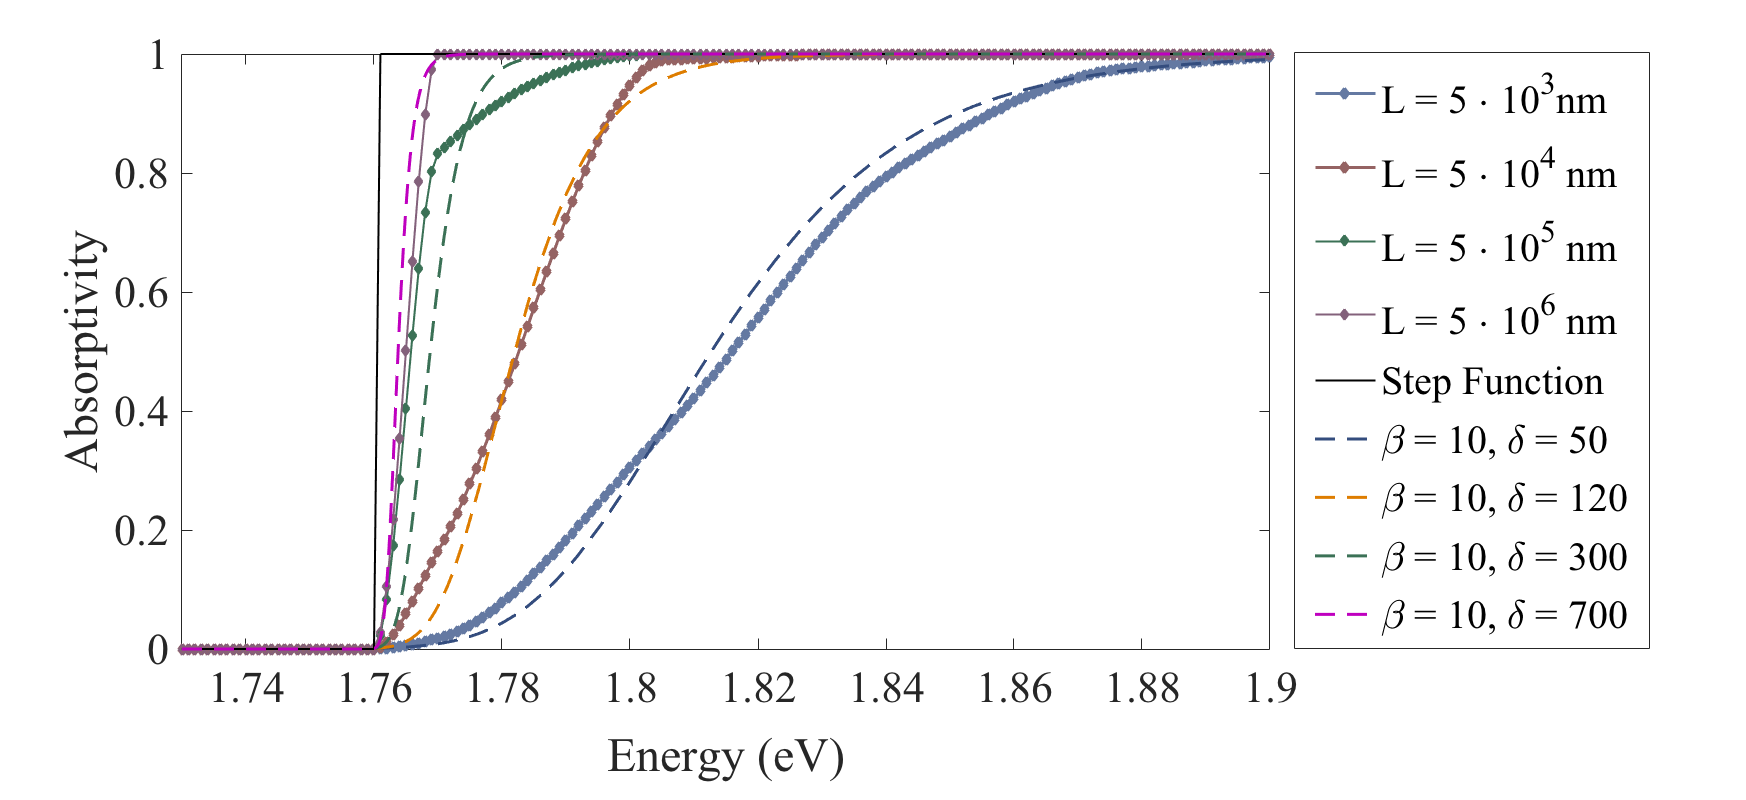
\includegraphics[width=0.8\textwidth]{Figures/slme/sq_Fig2.png} 
\caption{Comparison of the model function with calculated absorptivity spectra 
for \ce{Cu2ZnGeS4} at different thicknesses $L$. The model function shape 
matches that of the calculated absorptivity quite well as $L,\delta 
\rightarrow \infty$.} 
\label{fig:slme-step} 
\end{figure} 
 
To study the influence of the band gap on the likelihood of the efficiency 
exceeding the Shockley-Queisser limit, we calculate the efficiency for $\delta 
\in [1, 10^4]$ over the band gap range $E_g~\in~[0.3, 3]~\si{\electronvolt}$. 
We show the $\delta$-dependency of the efficiency for a selection of band gap 
values in Fig.~\ref{fig:slme-deltadep}. We can see that for low band gaps, the 
calculated efficiency crosses the detailed balance limit of the corresponding 
band gap, in order to return to the limit value for $\delta \rightarrow 
\infty$. Since $\delta$ can be related to the thickness of the material, this 
implies that for lower band gap materials, there is a thickness that is 
optimal for the efficiency. Moreover, a clear trend is visible, with the 
efficiency exceeding the Shockley-Queisser limit more as the band gap is 
decreased. This is also what we observe when we look at the plot for the 
maximum efficiency values in Fig.~\ref{fig:slme-SLME}. 
 
\begin{figure}[h!] 
\centering 
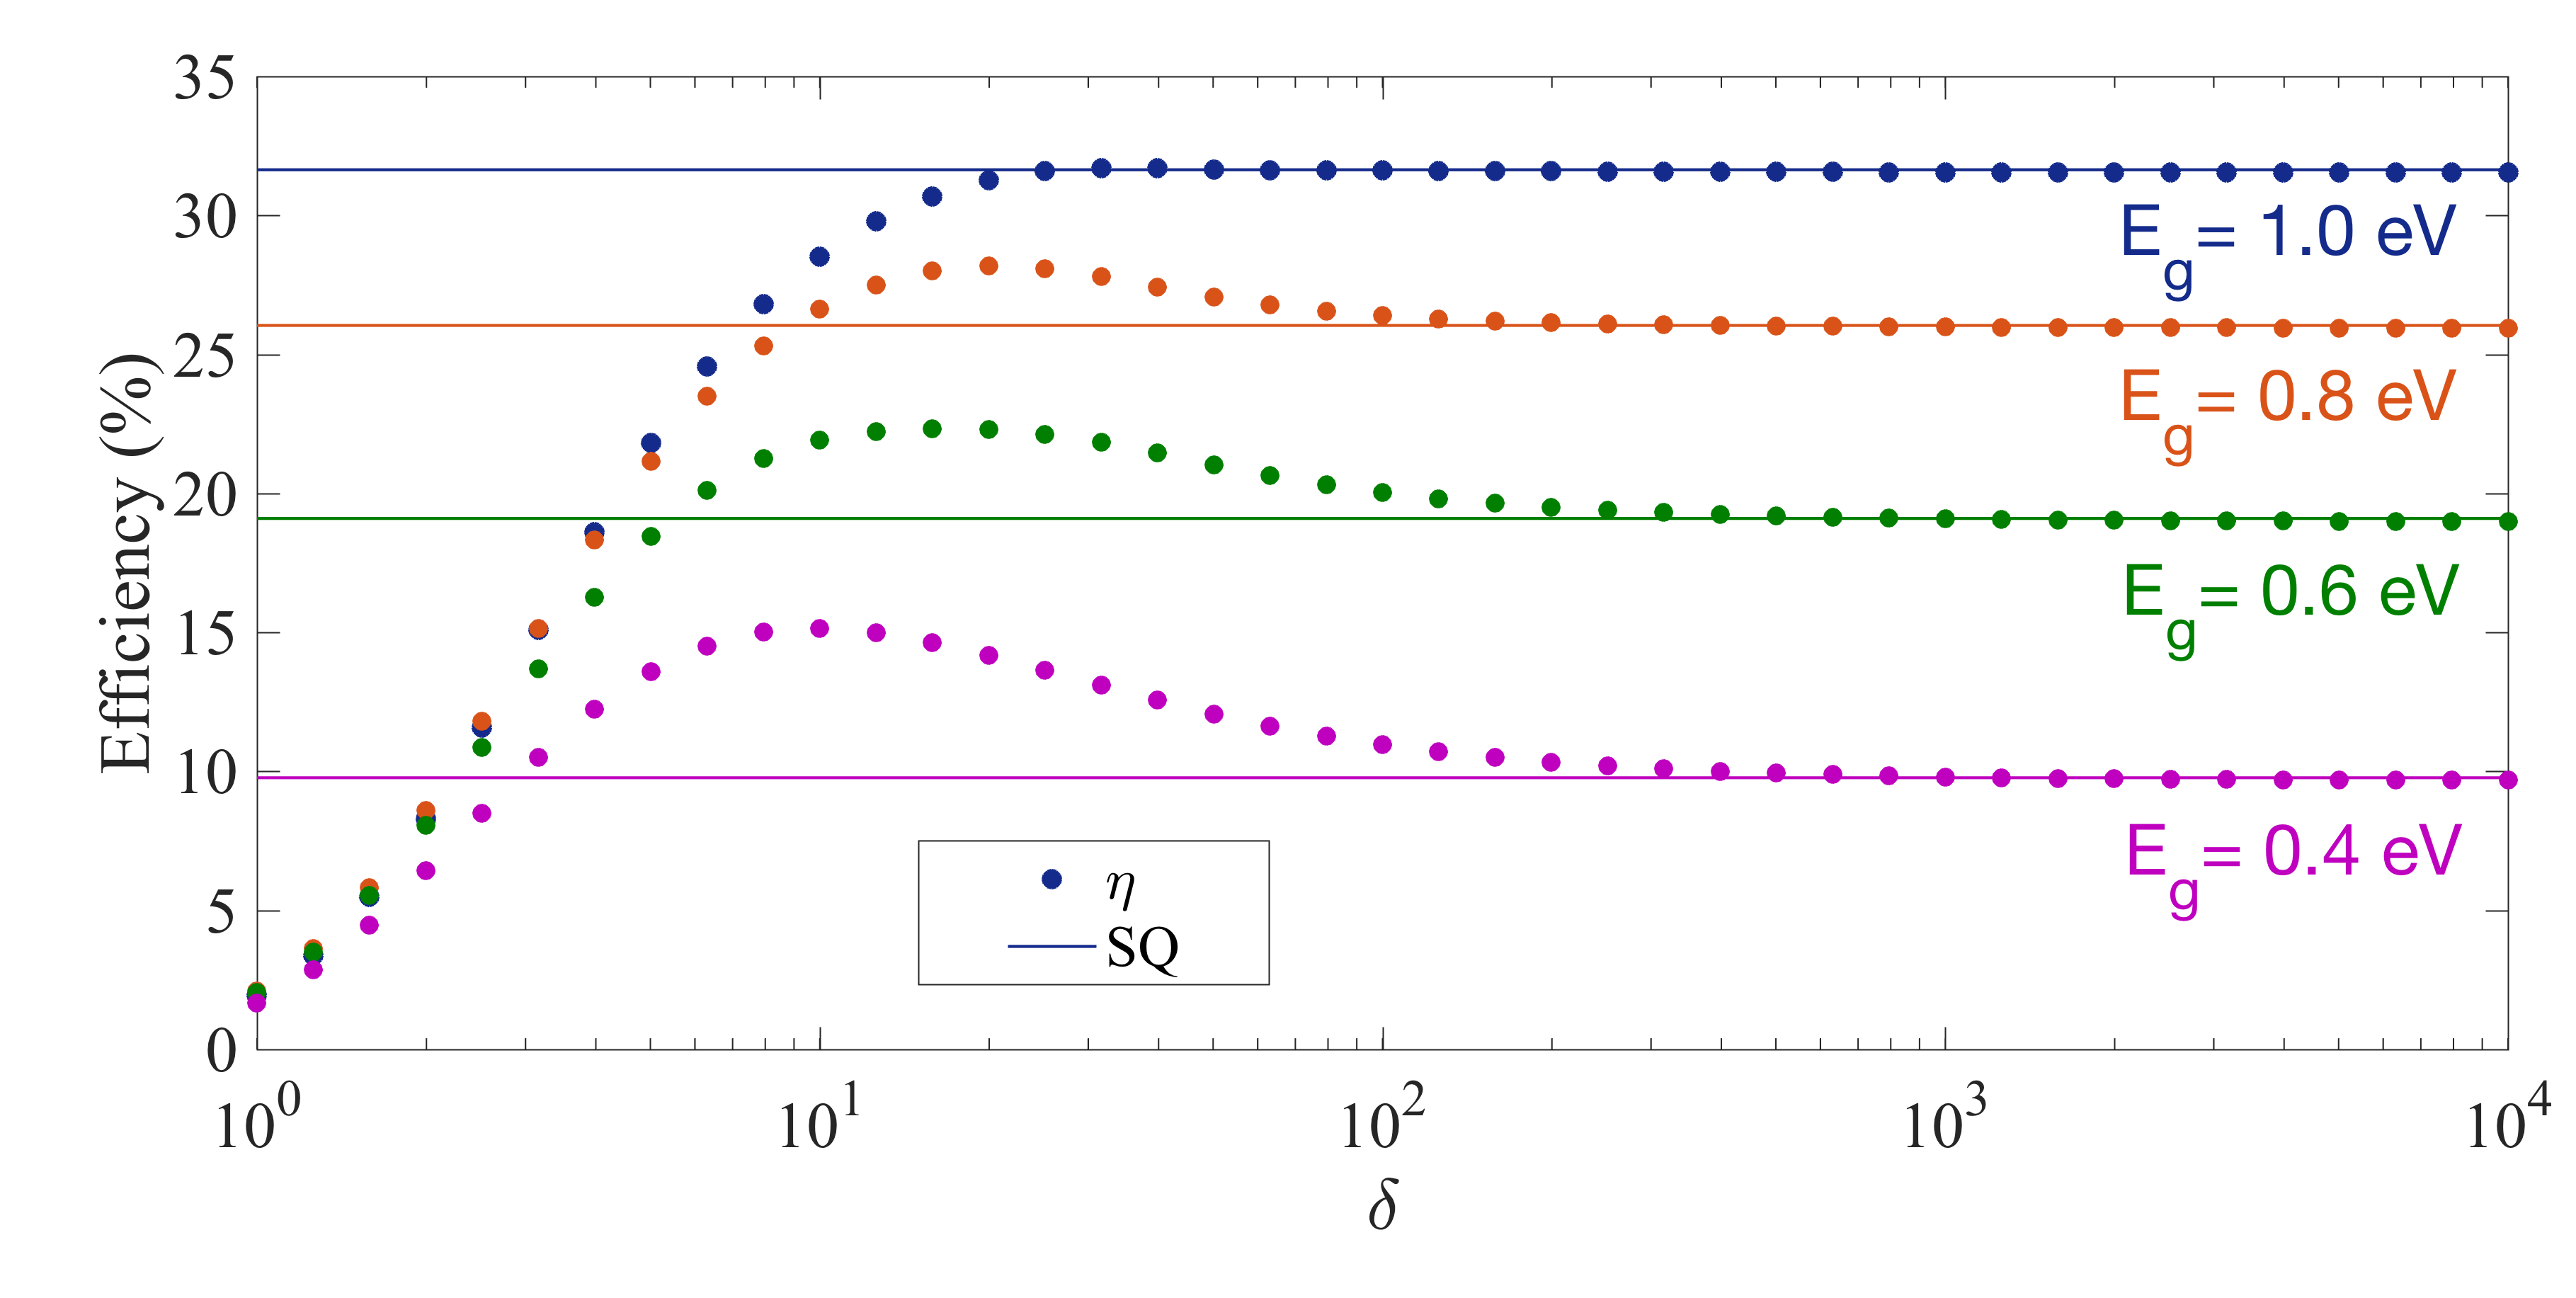
\includegraphics[width=0.8\textwidth]{Figures/slme/sq_Fig3.png} 
\caption{Calculated efficiencies for a range of $\delta$ values and a 
selection of band gaps, compared with the corresponding Shockley-Queisser 
limit.} 
\label{fig:slme-deltadep} 
\end{figure} 
 
Finally, it is interesting to note that the SLME values of the materials that 
exceed the Shockley-Queisser limit are still below the maximum efficiency for 
the model absorptivity functions of the corresponding band gap in 
Fig.~\ref{fig:slme-SLME}. However, this does not imply that the logistic 
function maxima curve represents a new upper limit. It is entirely possible 
that there is another function profile that would allow for higher 
efficiencies. Using the logistic function approach, we are simply able to 
observe for which band gap range the Shockley-Queisser limit does not provide 
a theoretical upper limit within the detailed balance approach. 
 
\subsection{Indirect band gap absorbers} 
 
So far, we have only considered materials which have a direct band gap. In 
order to test the application of the SLME to indirect band gap absorbers, we 
choose to calculate the SLME of silicon, which is still one of the most 
popular materials for the production of solar cells. In 
Fig.~\ref{fig:slme-Si_expAbs}, we show the experimental\footnote{We choose to 
use an experimental spectrum in order to include the phonon-mediated 
contributions to the absorption coefficient.} absorption coefficient of 
crystalline silicon~\cite{green2008}. Notice the onset of the indirect and 
direct absorption at \mbox{$E_g = 1.17~\si{\electronvolt}$} and 
\mbox{$E_g^{da} = 3.4~\si{\electronvolt}$}, respectively. 
 
\begin{figure}[htbp] 
	\centering 
		\includegraphics[width=0.7\textwidth]{./Figures/slme/Fig10.png} 
	\caption{Experimental absorption coefficient at $T = 300\si{\kelvin}$ of 
crystalline silicon with data taken from~\cite{green2008}.} 
	\label{fig:slme-Si_expAbs} 
\end{figure} 
 
Calculating the SLME using this optical spectrum produces an efficiency of 
zero for any value of $L$ and $T$. The origin of this troubling result is 
rooted in the fraction of radiative recombination expressed in 
Eq.~(\ref{eq:slme-fraction}). Because of the large difference between the 
direct allowed and fundamental band gap of silicon ($\Delta = 
E_g^{da}-E_g=2.23$~\si{\electronvolt}), the radiative fraction is of the order 
$10^{-38}$. Since this fraction is used to calculate the reverse saturation 
current (see Eq.~(\ref{eq:slme-currents})), this results in a $J_0$ that is 
unreasonably large. As discussed in Section~\ref{sec:slme-CuAu}, $J_0$ has a 
significant influence on the open circuit voltage $V_{oc}$. In this case, the 
high value of $J_0$ leads to a $V_{oc}$ that is too small to produce any 
significant power density. However, in case we set \mbox{$f_r = 10^{-3}$}, a 
more reasonable value for silicon~\cite{Shockley1952,Trupke2003,Richter2012}, 
then we obtain the results shown in Fig.~\ref{fig:slme-SLME_Si}. 
 
\begin{figure}[htbp] 
	\centering 
		\includegraphics[width=0.7\textwidth]{./Figures/slme/Fig11.png} 
	\caption{Thickness dependence of the SLME of silicon.} 
	\label{fig:slme-SLME_Si} 
\end{figure} 
 
One could argue that silicon is a special case, and that generally efficient 
indirect absorbers do not have such a large band gap difference \mbox{$\Delta 
= E_g ^{da}- E_g$}. For thin-film solar cells, indirect absorption also 
contributes significantly less to the power density. Consequently, indirect 
band gap materials with a large fundamental band gap are not suitable for 
these applications in any case. However, even for materials with a small 
$\Delta$, the modeled fraction of radiative recombination quickly becomes 
minute. For example, consider the compound Cu$_3$TlSe$_2$, which has been 
investigated by Yu and Zunger~\cite{Yu2012}. The reported difference between 
the fundamental and direct allowed band gap is $0.24$~\si{\electronvolt}. At 
300~\si{\kelvin}, the fraction of radiative recombination then becomes 
\mbox{$f_r = 10^{-4}$}. This means that although $99.99$~\% of the 
recombination is non-radiative in nature, the reverse saturation current is 
still derived from an entirely radiative principle, based on the black-body 
spectrum in Eq.~(\ref{eq:slme-currents}). Furthermore, it is clear that 
because of the exponential function in Eq.~(\ref{eq:slme-fraction}), the 
fraction of radiative recombination drops very rapidly with increasing 
$\Delta$. This indicates that even for materials with a relatively low 
$\Delta$, the reverse saturation current will rise significantly, which is 
detrimental for the calculated efficiency. Hence, it is entirely possible that 
the recombination model of the SLME metric does not judge indirect band gap 
absorbers fairly, potentially eliminating good materials during the selection 
procedure.\\ 
 
\section{Conclusion} 
 
We have compared the structural and thermodynamic properties of the CA and CH 
phase of the compounds. By analyzing the difference in formation energy of the 
CH and CA phase, we conclude that CA domains are most likely to be present in 
\mbox{CuIn-VI$_2$} compounds, which is in good agreement with experimental 
results. From the calculated optoelectronic properties of the materials, we 
have determined their potential as absorbers for solar cells by applying the 
SLME selection metric. We identify several compounds with a high theoretical 
efficiency in the CA phase, most notably \mbox{CA-CuInS$_2$}, which has a 
significantly higher efficiency than the corresponding CH phase. 
 
After observing an SLME value above the Shockley-Queisser limit for 
\mbox{CA-CuInSe$_2$}, we have performed a detailed analysis to find the origin 
of this result. We find that, within the details balance approach, the reverse 
saturation current $J_0$ approaches its SQ value very slowly for an increasing 
thickness $L$. This causes the SLME to cross the SQ limit for materials with a 
$J_0$ that is relatively high, i.e. materials with a low band gap or at higher 
temperatures. In their 1961 paper, Shockley and Queisser characterized their 
calculated efficiency as an upper limit, because of the assumption that if 
every photon with an energy above the band gap is absorbed, the obtained 
efficiency must be maximal. Although this assumption may seem entirely 
sensible at first glance, it does not consider the fact that it also maximizes 
the recombination current, which is calculated using the detailed balance 
principle. Because an increased recombination results in a lower efficiency, 
this means that lowering the absorptivity can produce higher efficiencies than 
the Shockley-Queisser limit under the right conditions. By using a model 
absorptivity function, which closely resembles absorptivity spectra calculated 
from first principles, we have shown that this can occur for low band gaps. 
This means that one must take care when dismissing low band gap materials 
based on their Shockley-Queisser limit, for their actual efficiency at certain 
thicknesses might still make them suitable for thin film photovoltaic 
applications. Finally, we show that the model that introduces non-radiative 
recombination to the SLME quickly undercuts the efficiency of indirect band 
gap absorbers, as the Boltzmann factor used increases the recombination 
current drastically once the difference between the direct and fundamental 
band gap becomes larger. 
 
\printbibliography 
\end{refsection} 